\documentclass[11pt,letterpaper]{article}

% --- PAQUETES FUNDAMENTALES ---
\usepackage[utf8]{inputenc}
\usepackage[spanish,es-tabla]{babel}
\usepackage{amsmath,amssymb}
\usepackage{graphicx}
\usepackage{geometry}
\usepackage{fancyhdr}
\usepackage{booktabs}
\usepackage{tabularx}
\usepackage{multirow}
\usepackage{colortbl}
\usepackage{xcolor}
\usepackage{tcolorbox}
\usepackage{caption}
\usepackage{subcaption}
\usepackage{float}
\usepackage{titlesec}
\usepackage{enumitem}
\usepackage{hyperref}

% --- CONFIGURACIÓN DE PÁGINA ---
\geometry{
    top=2.5cm,
    bottom=2.5cm,
    left=2.5cm,
    right=2.5cm,
    headheight=15pt,
    footskip=1.2cm
}

% --- COLORES CORPORATIVOS CCCD / IEJAGA ---
\definecolor{navyiejaga}{RGB}{28,69,135}    % #1C4587
\definecolor{darkslate}{RGB}{38,50,56}     % #263238
\definecolor{rojorocket}{RGB}{194,24,91}    % #C2185B
\definecolor{verdecumple}{RGB}{46,125,50}   % #2E7D32
\definecolor{grisclaro}{RGB}{245,247,250}   % #F5F7FA
\definecolor{bordeazul}{RGB}{160,185,220}

% --- ESTILO DE TÍTULOS ---
\titleformat{\section}
  {\normalfont\large\bfseries\color{navyiejaga}\centering}{\thesection.}{0.5em}{\MakeUppercase}
  [\vspace{0.1cm}\titlerule]

\titleformat{\subsection}
  {\normalfont\normalsize\bfseries\color{navyiejaga}}{\thesubsection.}{0.5em}{}

\titleformat{\subsubsection}
  {\normalfont\small\bfseries\color{navyiejaga}}{\thesubsubsection.}{0.5em}{}

\titlespacing*{\section}{0pt}{14pt}{8pt}
\titlespacing*{\subsection}{0pt}{10pt}{4pt}
\titlespacing*{\subsubsection}{0pt}{8pt}{3pt}

% --- ENCABEZADOS Y PIES DE PÁGINA ---
\pagestyle{fancy}
\fancyhf{}
\fancyhead[L]{\small\color{gray}\textbf{CCCD 2026} --- Concurso Colombiano de Cohetería Deportiva}
\fancyhead[R]{\small\color{navyiejaga}\textbf{Equipo 211: PDA Stars}}
\fancyfoot[L]{\small\color{gray}Critical Design Review (CDR) --- Categoría 2 (Intermedios)}
\fancyfoot[R]{\small\bfseries\color{navyiejaga}\thepage}
\renewcommand{\headrulewidth}{0.6pt}
\renewcommand{\footrulewidth}{0.4pt}

% --- HIPERVÍNCULOS ---
\hypersetup{
    colorlinks=true,
    linkcolor=navyiejaga,
    citecolor=navyiejaga,
    urlcolor=navyiejaga,
    pdftitle={Critical Design Review - Equipo 211 PDA Stars - CCCD 2026},
    pdfauthor={I.E. José Antonio Galán - Semillero PDA},
    pdfsubject={Cohete Deportivo PDA Stars - Categoría 2 (Motor F15-4)}
}

% --- COMANDO PARA ESPACIO DE FOTOS FALTANTES (PLACEHOLDER) ---
\newcommand{\placeholderbox}[2]{%
  \begin{figure}[H]
    \centering
    \begin{tcolorbox}[width=0.92\linewidth, colback=grisclaro, colframe=navyiejaga!60!black, boxrule=1pt, arc=3pt, halign=center, valign=center]
      \vspace{0.3cm}
      {\color{navyiejaga}\normalsize\bfseries\textsf{[ESPACIO RESERVADO PARA REGISTRO FOTOGRÁFICO / EVIDENCIA EN TALLER]}}\\[0.2cm]
      {\small\color{darkslate}#2}\\[0.2cm]
      {\scriptsize\color{gray}\textit{(Para insertar la imagen definitiva en el código fuente, reemplace este entorno por el archivo fotográfico correspondiente en la carpeta figures/)}}
      \vspace{0.3cm}
    \end{tcolorbox}
    \vspace{-0.2cm}
    \caption{#2}
  \end{figure}
}

% --- RUTA DE IMÁGENES ---
\graphicspath{{figures/}}

\begin{document}

% 0. PORTADA
\begin{titlepage}
\centering
\vspace*{0.5cm}

% Logotipos superiores
\begin{figure}[H]
\centering

\includegraphics[height=1.8cm]{logo_header.png}
\end{figure}

\vspace{0.8cm}
{\color{navyiejaga}\Large\textbf{CONCURSO COLOMBIANO DE COHETERÍA DEPORTIVA}}\\[0.2cm]
{\color{navyiejaga}\large\textbf{CCCD 2026}}\\[0.4cm]
{\color{darkslate}\textbf{CATEGORÍA 2: POTENCIA MEDIA (INTERMEDIOS) --- MOTOR F15-4}}\\[0.8cm]

\rule{\linewidth}{1.2pt}\\[0.4cm]
{\color{navyiejaga}\LARGE\textbf{CRITICAL DESIGN REVIEW (CDR)}}\\[0.3cm]
{\color{rojorocket}\Large\textbf{PROYECTO PDA STARS --- EQUIPO ID: 211}}\\[0.2cm]
{\large\textit{Documento de Revisión Crítica de Diseño y Evaluación Técnica de Misión}}\\[0.2cm]
\rule{\linewidth}{1.2pt}\\[1.0cm]

\begin{figure}[H]
\centering

\includegraphics[width=4.5cm]{parche_mision.png}
\end{figure}

\vfill

\begin{minipage}{0.48\linewidth}
\raggedright
\textbf{Institución Educativa:}\\
I.E. José Antonio Galán\\
Municipio de La Estrella, Antioquia\\
Semillero de Investigación PDA
\end{minipage}
\hfill
\begin{minipage}{0.48\linewidth}
\raggedleft
\textbf{Equipo Técnico 211:}\\
Líder: Samuel Gómez Correa\\
Director: Docente Asesor Técnico\\
Fecha de Radicación: Octubre de 2026
\end{minipage}

\vspace{0.8cm}
\begin{center}

\includegraphics[height=1.2cm]{logo_cccd.png}\hspace{1.5cm}

\includegraphics[height=1.2cm]{logo_iejaga.png}\hspace{1.5cm}

\includegraphics[height=1.2cm]{logo_pda.png}
\end{center}

\end{titlepage}

\newpage

% ÍNDICE GENERAL
{
  \hypersetup{linkcolor=darkslate}
  \tableofcontents
  \newpage
  \listoffigures
  \vspace{0.5cm}
  \listoftables
}
\newpage

% 1. PARCHE DE MISIÓN
\section{Parche de Misión}

El parche de misión de \textbf{PDA STARS} representa la identidad científica, la disciplina ingenieril y el espíritu de innovación del semillero aeroespacial de la Institución Educativa José Antonio Galán (La Estrella, Antioquia) en el Concurso Colombiano de Cohetería Deportiva 2026.

\begin{figure}[H]
\centering

\includegraphics[width=0.42\linewidth]{parche_mision.png}
\caption{Parche oficial de la misión PDA STARS (Equipo 211).}
\label{fig:parche_mision}
\end{figure}

\subsection{Significado y Simbolismo Técnico}
\begin{itemize}[leftmargin=1.5em]
    \item \textbf{El Cohete en Ascenso:} Simboliza el desarrollo estructural, la propulsión eficiente con el motor oficial Estes F15-4 y la precisión requerida para alcanzar el apogeo reglamentario de 300 metros con trayectoria vertical estable.
    \item \textbf{Las Estrellas:} Rinden tributo al municipio de La Estrella (cuna del equipo) y a las metas de excelencia científica trazadas por los estudiantes galanistas.
    \item \textbf{La Órbita y Estela:} Representan la integración interdisciplinaria entre la física atmosférica, la simulación computacional de vuelo, la instrumentación electrónica de la carga útil y la recuperación segura.
    \item \textbf{La Paleta Cromática:} El azul institucional refleja la serenidad y rigor analítico; el dorado evoca la calidad y perseverancia en las pruebas experimentales; el rojo personifica la energía de la combustión del grano sólido y la pasión investigativa.
\end{itemize}


% 2. EQUIPO DE MISIÓN
\section{Equipo de Misión}

La misión PDA STARS está conformada por un equipo interdisciplinario de estudiantes y asesores técnicos de la I.E. José Antonio Galán, organizados bajo una estructura funcional con roles claramente delimitados conforme a las normativas del concurso.

\begin{figure}[H]
\centering
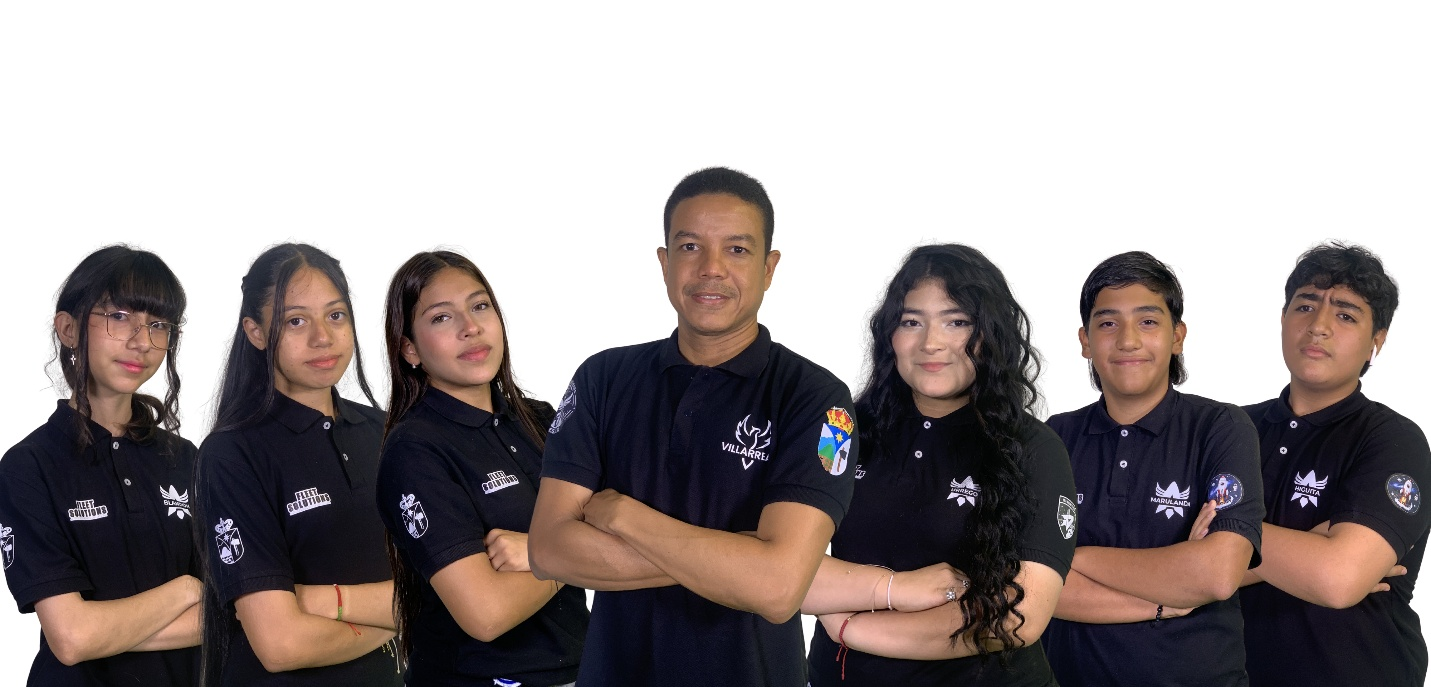
\includegraphics[width=0.75\linewidth]{equipo_mision.jpg}
\caption{Fotografía del equipo oficial PDA STARS (Equipo 211).}
\label{fig:equipo_mision}
\end{figure}

\subsection{Estructura Organizacional y Roles Técnicos}
\begin{table}[H]
\centering
\small
\begin{tabularx}{\linewidth}{p{4.2cm}p{3.5cm}X}
\toprule
\rowcolor{navyiejaga!15}
\textbf{Miembro / Rol} & \textbf{Responsabilidad Principal} & \textbf{Área Técnica Asignada} \\
\midrule
\textbf{Líder de Misión} & Samuel Gómez Correa & Coordinación general, cronograma de hitos, integración interdisciplinaria y vocería técnica. \\
\rowcolor{grisclaro}
\textbf{Diseño y Aerodinámica} & Responsable Técnico & Simulación digital OpenRocket, modelado CAD 3D de aletas y ojiva Haack, optimización del margen estático ($CG/CP$). \\
\textbf{Estructura y Materiales} & Responsable Técnico & Mecanizado de tubos Kraft BT-80, manufactura aditiva FDM en filamentos PETG/PETG-CF, acoples y ensamble estructural. \\
\rowcolor{grisclaro}
\textbf{Propulsión y Recuperación} & Responsable Técnico & Montaje del tubo portamotor 29 mm, cálculo de retardos, dimensionamiento del paracaídas ripstop de 40 cm y manta Nomex. \\
\textbf{Carga Útil y Aviónica} & Responsable Técnico & Programación de microcontrolador Seeeduino XIAO, integración de sensores DPS310/MPU6050, diseño PCB y telemetría. \\
\rowcolor{grisclaro}
\textbf{Oficial de Seguridad (RSO)} & Responsable Técnico & Verificación de listas de chequeo en rampa, inspección pre-vuelo, cumplimiento de radios de exclusión y gestión de riesgos. \\
\bottomrule
\end{tabularx}
\caption{Organigrama de responsabilidades del equipo PDA STARS.}
\label{tab:roles_equipo}
\end{table}


% 3. REQUERIMIENTOS Y RESTRICCIONES
\section{Requerimientos y Restricciones}

El diseño, construcción, simulación y operación del cohete PDA STARS se rigen estrictamente por los reglamentos oficiales de la Categoría 2 (Intermedios) del CCCD 2026, el Documento de Diseño, Construcción y Pruebas (DCP) y la Norma de Seguridad en Cohetería Deportiva (NSRT).

\subsection{Requerimientos de la Misión}
\begin{itemize}[leftmargin=1.5em]
    \item \textbf{Cota de Altura Objetivo:} Alcanzar un apogeo vertical lo más cercano posible a exactamente \textbf{300 metros} sobre el nivel del terreno de lanzamiento.
    \item \textbf{Ventana de Tiempo de Vuelo:} Mantener una duración total de vuelo (desde la ignición hasta el aterrizaje) comprendida entre \textbf{40 y 50 segundos}, correspondiente a la exigencia oficial para cohetes propulsados por motores de clase F.
    \item \textbf{Recuperación Íntegra en Zona Segura:} El vehículo debe desplegar su paracaídas tras el apogeo y aterrizar completamente intacto dentro del radio de exclusión oficial de \textbf{250 metros} alrededor de la rampa de lanzamiento.
\end{itemize}

\subsection{Requerimientos del Sistema}
\begin{itemize}[leftmargin=1.5em]
    \item \textbf{Dimensiones Estructurales:} Longitud total de \textbf{68,5 cm} (685 mm) y diámetro exterior de fuselaje de \textbf{66,0 mm} (correspondiente al tubo comercial Kraft BT-80).
    \item \textbf{Masa de Vuelo:} Masa total del cohete en rampa estimada en \textbf{528 gramos} (con motor cargado e instrumentación a bordo), no excediendo el límite estructural máximo de 650 g establecido para la categoría.
    \item \textbf{Módulos Intercambiables:} Arquitectura seccionada en tres cuerpos acoplables: ojiva desmontable, contenedor cilíndrico de electrónica/carga útil y fuselaje propulsor principal.
\end{itemize}

\subsection{Requerimientos de Propulsión y Carga Útil}
\begin{itemize}[leftmargin=1.5em]
    \item \textbf{Motor Oficial Homologado:} Uso exclusivo del motor comercial de combustible sólido \textbf{Estes F15-4} (diámetro 29 mm, longitud 114 mm, impulso total 49,6 N·s, retardo de eyección de 4 segundos).
    \item \textbf{Masa de Carga Útil:} Carga útil científica experimental con una masa de exactamente \textbf{60,0 gramos}, cumpliendo de manera estricta con la restricción de masa $\le 60\text{ g}$.
    \item \textbf{Medición Atmosférica e Inercial:} La carga útil debe registrar autónomamente perfiles de presión barométrica, altitud relativa calculada, temperatura ambiental y aceleración en 3 ejes a una frecuencia mínima de 10 Hz, con almacenamiento local en tarjeta microSD y respaldo no volátil en EEPROM.
\end{itemize}

\subsection{Requerimientos de Estructura y Aerodinámica}
\begin{itemize}[leftmargin=1.5em]
    \item \textbf{Estabilidad Aerodinámica Pasiva:} Margen estático mínimo obligatorio de \textbf{2,00 calibres} en la rampa de lanzamiento ($CP - CG \ge 13,2\text{ cm}$) conforme a la Sección 3.1.1 del DCP y Sección 4.3 de la NSRT.
    \item \textbf{Selección de Materiales Aprobados:} Fuselaje en tubo Kraft enrollado en espiral, ojiva en filamento PETG estándar (para garantizar permeabilidad electromagnética y evitar jaulas de Faraday), aletas y anillos de centrado en filamento PETG reforzado con fibra de carbono (PETG-CF) para máxima rigidez torsional.
\end{itemize}

\subsection{Restricciones Operativas y de Seguridad}
\begin{itemize}[leftmargin=1.5em]
    \item \textbf{Guía de Rampa:} Despegue desde varilla estándar de \textbf{1,5 metros} de longitud y $\varnothing 6,5\text{ mm}$ (1/4 in). La velocidad al abandonar la guía debe superar los \textbf{10,0 m/s} (36 km/h) para garantizar control aerodinámico inmediato.
    \item \textbf{Seguridad de Ignición:} Sistema de encendido eléctrico operado a distancia con llave física de enclavamiento, señal acústica previa de 5 segundos y radio de seguridad mínimo de \textbf{15 metros}.
\end{itemize}


% 4. CRONOGRAMA DE TRABAJO
\section{Cronograma de Trabajo}

Para garantizar el cumplimiento riguroso de los hitos del CCCD 2026, el equipo PDA STARS estructuró un plan de trabajo dividido en fases secuenciales: diseño preliminar, simulación aerodinámica, manufactura aditiva y mecánica, integración de aviónica, pruebas en tierra (estabilidad, eyección y banco de sensores), revisión crítica (CDR) y preparación para la campaña de lanzamiento.

\begin{figure}[H]
\centering
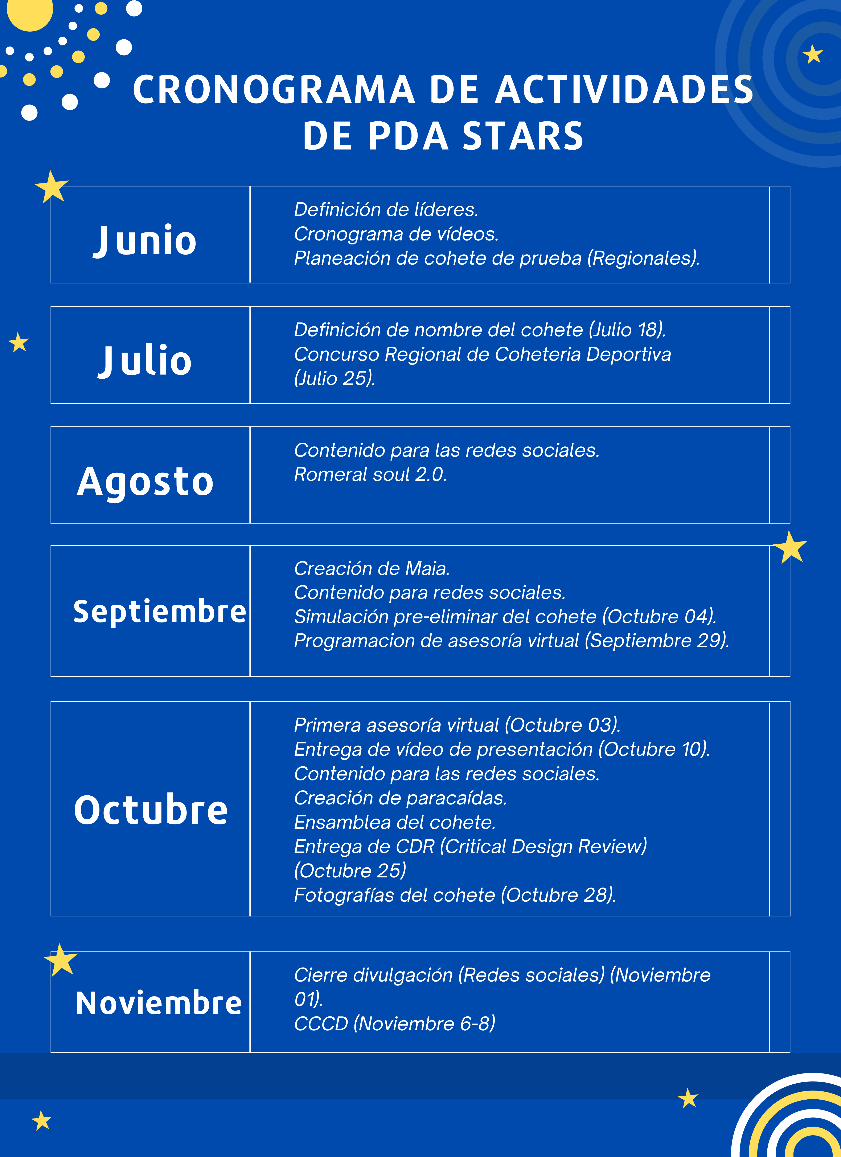
\includegraphics[width=0.95\linewidth]{cronograma_gantt.png}
\caption{Diagrama de Gantt y cronograma general de actividades del proyecto PDA STARS.}
\label{fig:cronograma_actividades}
\end{figure}

El cronograma evidencia la culminación exitosa de las fases de diseño y manufactura estructural, habiendo validado el margen de estabilidad en tierra y la respuesta de la carga útil experimental antes de la fecha límite de entrega de este reporte CDR.


% 5. ANÁLISIS DE DISEÑO DEL COHETE
\section{Análisis de Diseño del Cohete}

El diseño aerodinámico y estructural del vehículo PDA STARS se desarrolló mediante un proceso iterativo de modelado CAD tridimensional en Autodesk Fusion 360 y simulación aerodinámica en OpenRocket (archivo oficial \texttt{211\_PDASTARS\_Diseño.ork}), buscando satisfacer simultáneamente el requerimiento de apogeo a 300 m y la estabilidad pasiva $\ge 2,0\text{ cal}$.

\begin{figure}[H]
\centering
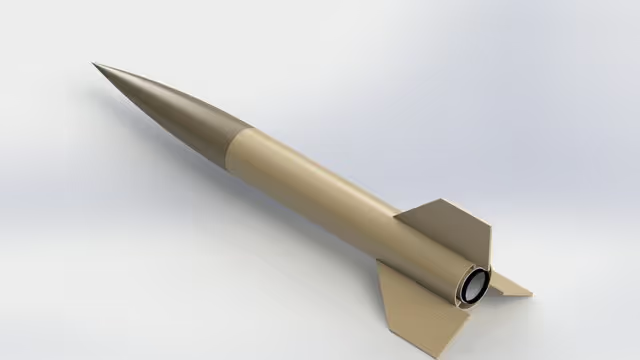
\includegraphics[width=0.75\linewidth]{cad_cohete.png}
\caption{Modelo digital tridimensional (CAD) del cohete PDA STARS en Fusion 360.}
\label{fig:cad_cohete}
\end{figure}

\subsection{Arquitectura Modular del Vehículo}
El cohete presenta una longitud total de \textbf{68,5 cm} (685 mm) y un diámetro exterior de \textbf{66,0 mm} (tubo Kraft comercial BT-80 con espesor de pared de 0,8 mm), dividido en tres módulos estructurales:
\begin{enumerate}[leftmargin=1.5em]
    \item \textbf{Ojiva Haack (Von Kármán):} Longitud de \textbf{13,0 cm}, fabricada mediante impresión FDM en filamento PETG sólido (masa de 39,7 g). Su perfil continuo optimiza la transición de presión en régimen subsónico compresible.
    \item \textbf{Bahía de Carga Útil y Aviónica:} Longitud de \textbf{19,0 cm} en tubo Kraft BT-80 (masa de 60,0 g). Aloja el contenedor impreso en 3D con el microcontrolador Seeeduino XIAO, sensores barométricos/inerciales, batería NiMH, altímetro digital y cáncamo estructural de retención.
    \item \textbf{Fuselaje Principal y Propulsión:} Longitud de \textbf{36,5 cm} en tubo Kraft BT-80 (masa de 30,0 g). Alberga el sistema de recuperación (paracaídas de 40 cm y manta Nomex de 15x15 cm), tubo portamotor concéntrico de 29 mm y 14,0 cm de longitud, dos anillos de centrado en PETG-CF y retén inferior roscado.
    \item \textbf{Conjunto de Aletas Estructurales:} Tres aletas de forma libre con perfil biconvexo sustentador (airfoil), envergadura de 12,0 cm, cuerda de raíz de 14,5 cm, cuerda de punta de 2,0 cm y espesor de 2,0 mm en PETG reforzado con fibra de carbono (PETG-CF, masa total del conjunto de 64,0 g), fijadas a través del fuselaje hasta el portamotor con resina epoxi de grado aeronáutico.
\end{enumerate}

\begin{figure}[H]
\centering
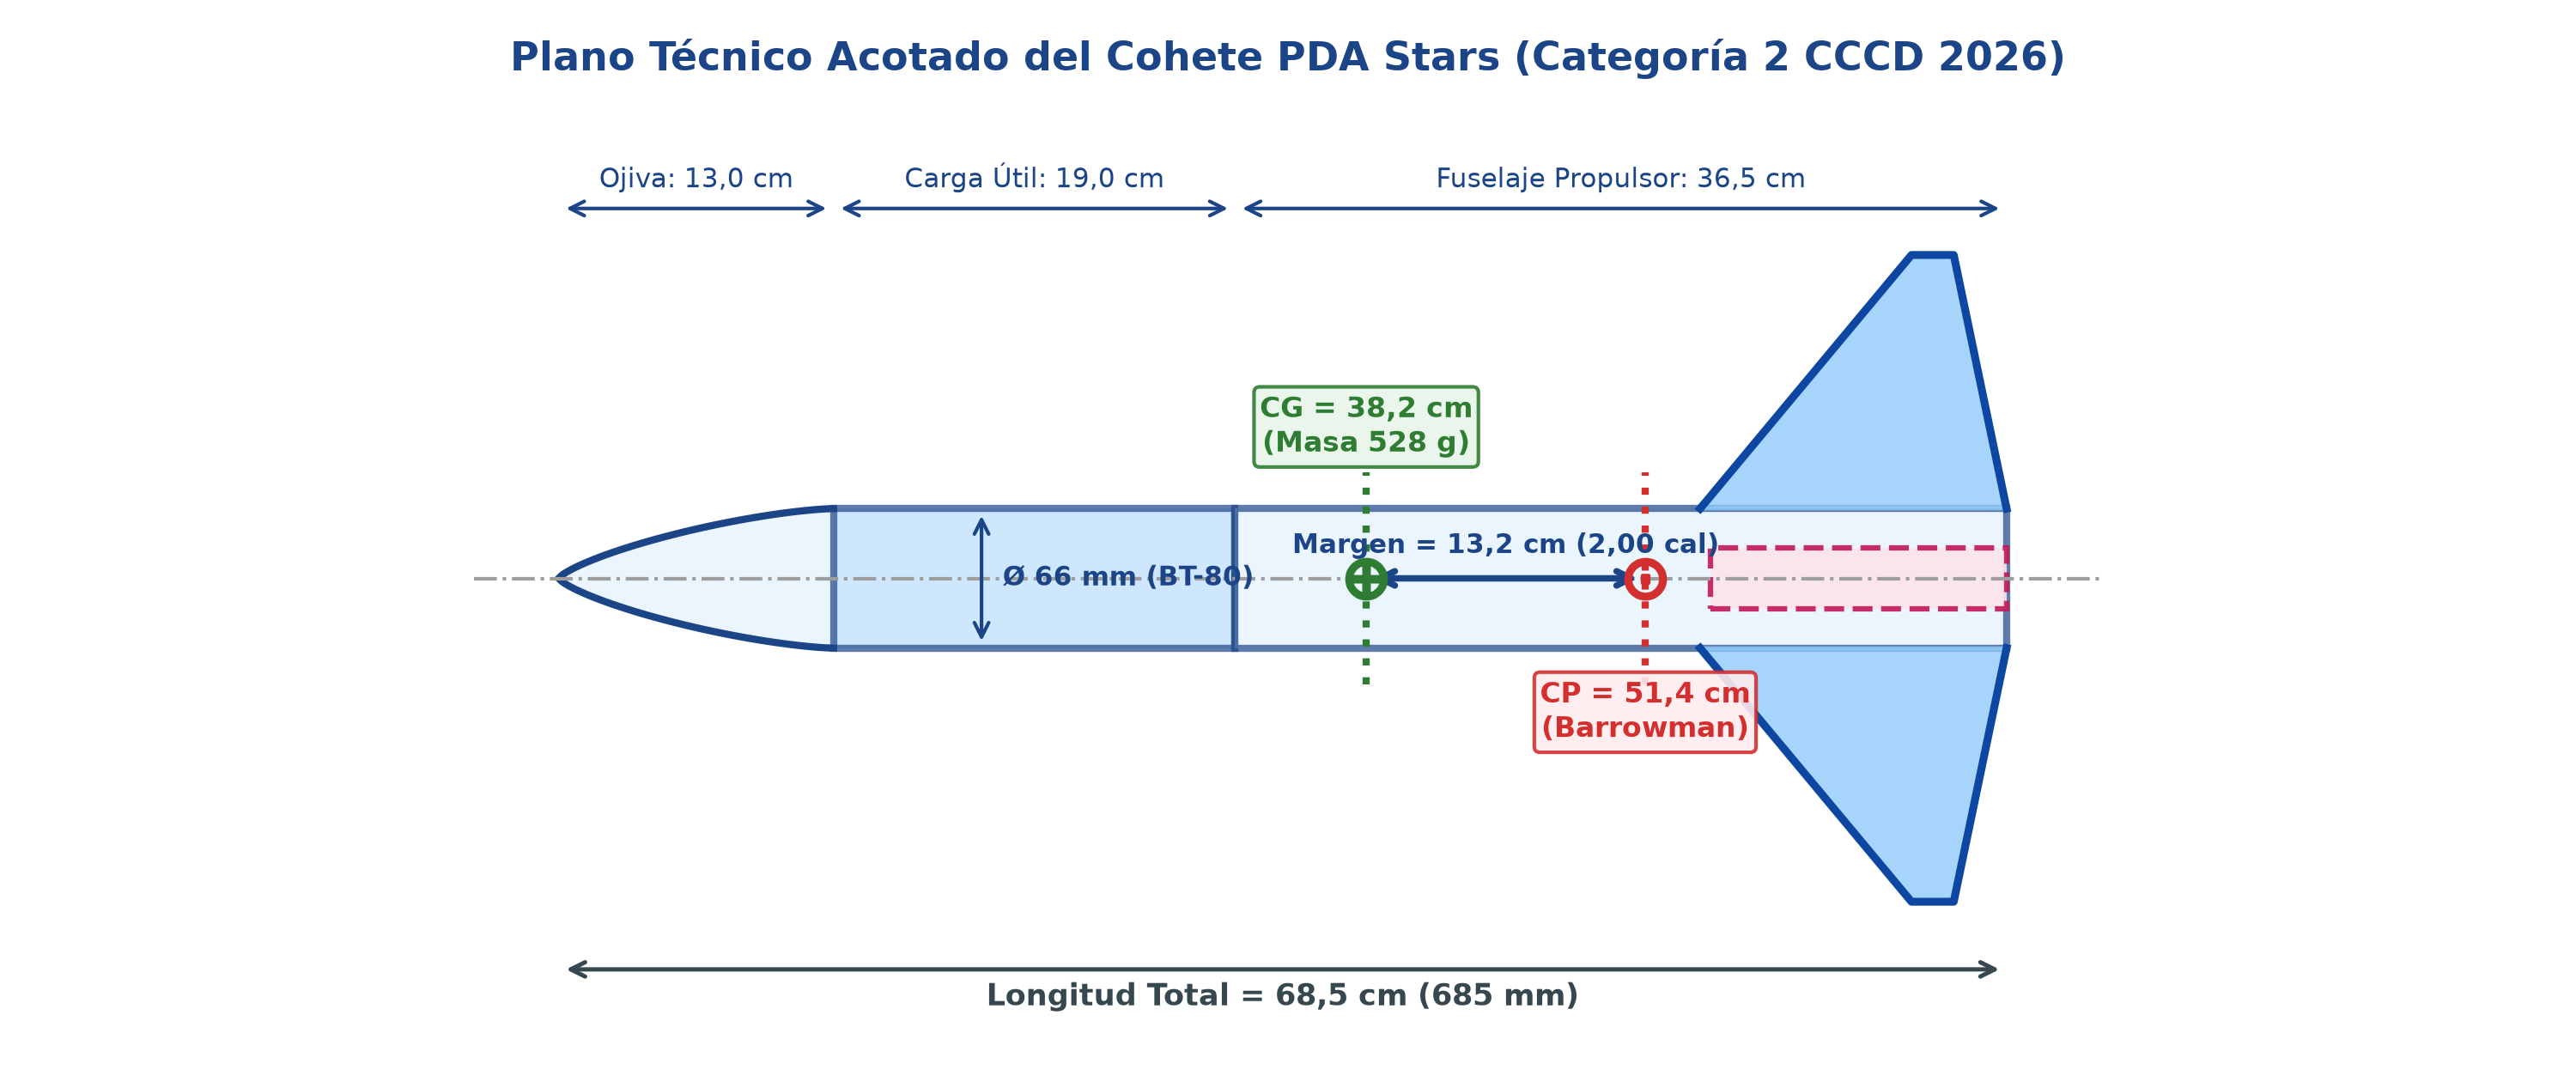
\includegraphics[width=0.95\linewidth]{fig_plano_acotado_cohete.png}
\caption{Plano técnico acotado y dimensionamiento estructural del cohete PDA STARS.}
\label{fig:plano_acotado}
\end{figure}

\begin{figure}[H]
\centering
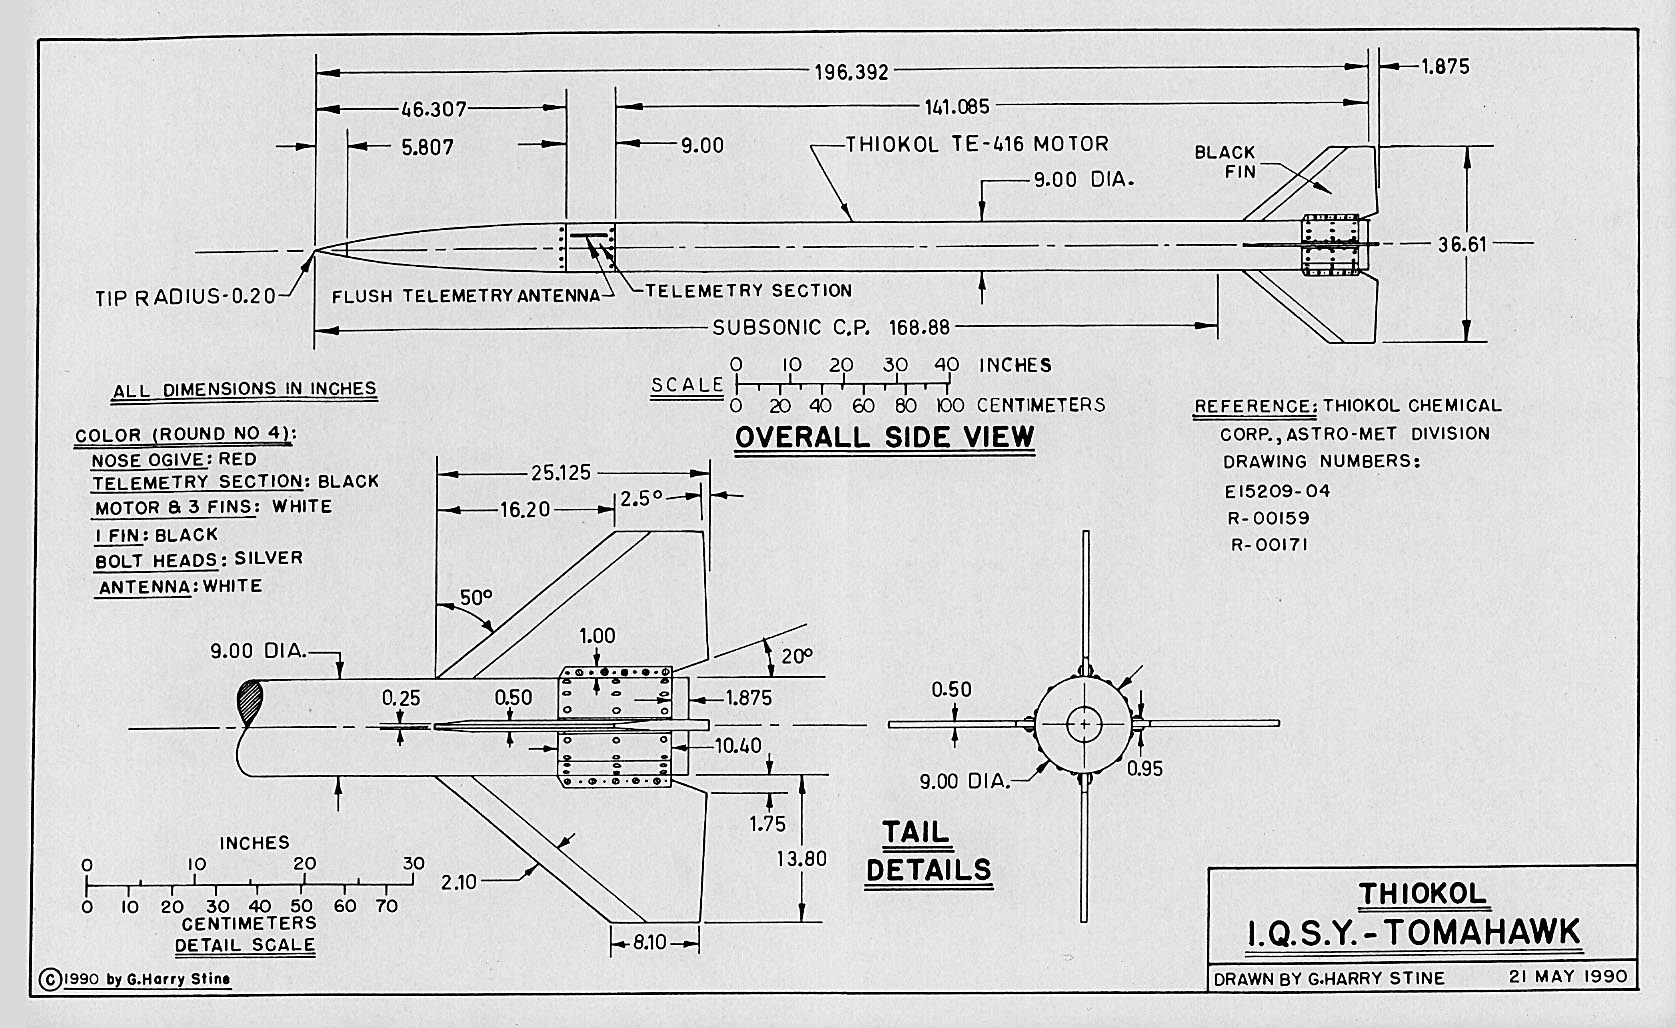
\includegraphics[width=0.85\linewidth]{plano_cohete.png}
\caption{Plano de conjunto y ensamble en software de diseño mecánico.}
\label{fig:plano_mecanico}
\end{figure}

\subsection{Distribución de Masas y Margen Estático de Estabilidad}
En la configuración definitiva de vuelo, el Centro de Gravedad real ($CG$) se ubica a \textbf{38,2 cm} desde el vértice de la ojiva con el vehículo totalmente cargado en rampa (masa total de 528 g). El Centro de Presión teórico ($CP$), calculado en OpenRocket mediante las formulaciones aerodinámicas clásicas de Barrowman, se sitúa a \textbf{51,4 cm}.

La separación estática resultante es de:
\begin{equation}
    \Delta x = CP - CG = 51,4\text{ cm} - 38,2\text{ cm} = 13,2\text{ cm}
\end{equation}
Expresado en función del calibre de referencia ($D = 6,6\text{ cm}$):
\begin{equation}
    \text{Margen Estático} = \frac{CP - CG}{D} = \frac{13,2\text{ cm}}{6,6\text{ cm}} = \mathbf{2,00\text{ calibres}}
\end{equation}
Durante la fase propulsada, a medida que el grano del motor Estes F15 se consume (60 g de propelente quemado), el $CG$ se desplaza ligeramente hacia adelante hasta los 37,8 cm, incrementando el margen estático a \textbf{2,05 calibres} en el momento del agotamiento (\textit{burnout}), lo cual garantiza un vuelo estrictamente estable en todas las etapas.


% 6. SIMULACIÓN DE VUELO
\section{Simulación de Vuelo}

La dinámica y trayectoria del cohete PDA STARS se verificaron mediante simulaciones numéricas en seis grados de libertad en OpenRocket, utilizando la curva de empuje certificada por NAR/TRA para el motor oficial Estes F15-4 (impulso total 49,6 N·s, empuje medio 14,8 N, tiempo de combustión nominal 3,4 s, retardo de eyección 4,0 s) y condiciones atmosféricas locales estándar (densidad del aire $\rho = 1,05\text{ kg/m}^3$ a 1700 msnm, viento cruzado de hasta 3,5 m/s).

\begin{figure}[H]
\centering
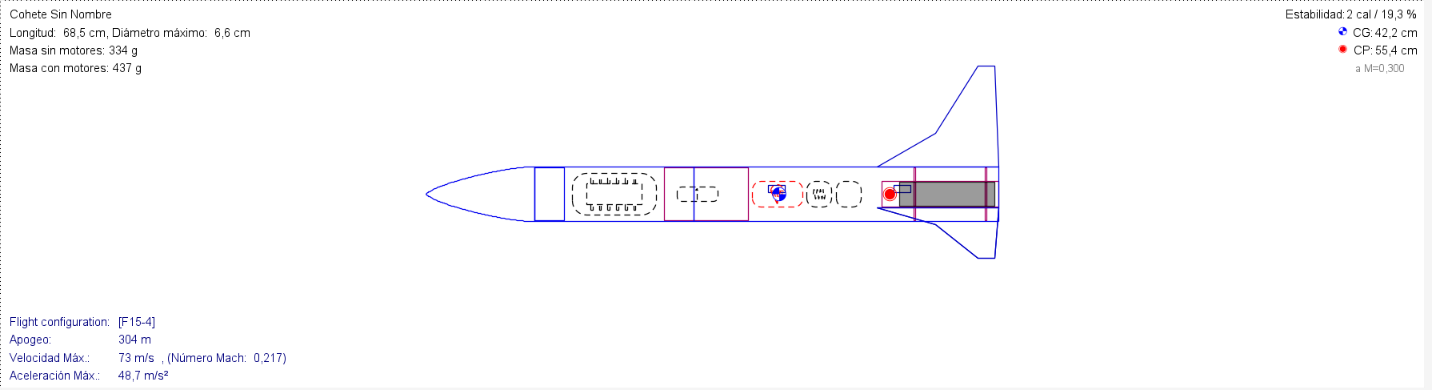
\includegraphics[width=0.85\linewidth]{vista_lateral_cohete.png}
\caption{Vista lateral y configuración de análisis aerodinámico del cohete PDA STARS.}
\label{fig:vista_lateral}
\end{figure}

\subsection{Resultados Numéricos Consolidados}
Los datos extraídos directamente de la simulación oficial (\texttt{simulacion\_stellaris.csv}) y el modelo \texttt{211\_PDASTARS\_Diseño.ork} confirman los siguientes parámetros de vuelo:

\begin{table}[H]
\centering
\small
\begin{tabularx}{\linewidth}{Xccp{4.5cm}}
\toprule
\rowcolor{navyiejaga!15}
\textbf{Parámetro de Vuelo} & \textbf{Valor Simulado} & \textbf{Límite / Meta CCCD} & \textbf{Estado de Cumplimiento} \\
\midrule
\textbf{Velocidad en salida de varilla ($1,5\text{ m}$)} & 10,70 m/s (38,5 km/h) & $\ge 10,0\text{ m/s}$ & Cumple (control aerodinámico inmediato) \\
\rowcolor{grisclaro}
\textbf{Aceleración vertical máxima} & 48,68 m/s² (4,96 G) & $< 15\text{ G}$ & Cumple (cargas tolerables en Kraft/epoxi) \\
\textbf{Velocidad máxima de ascenso} & 73,01 m/s (Mach 0,217) & Subsonico ($< 0,3$) & Cumple (baja resistencia compresible) \\
\rowcolor{grisclaro}
\textbf{Tiempo hasta el apogeo} & 8,90 s & Nominal 8--10 s & Cumple (trayectoria ascendente estable) \\
\textbf{Apogeo máximo alcanzado} & \textbf{304,22 m} & \textbf{300,0 m} & \textbf{Cumple} (desviación mínima de $+1,4\%$) \\
\rowcolor{grisclaro}
\textbf{Velocidad al abrir paracaídas} & 17,86 m/s (a los 8,5 s) & $< 25\text{ m/s}$ & Cumple (eyección segura cerca al apogeo) \\
\textbf{Velocidad terminal de descenso} & \textbf{8,00 m/s} ($7,998\text{ m/s}$) & $6,0\text{ -- }9,0\text{ m/s}$ & Cumple (aterrizaje sin impacto estructural) \\
\rowcolor{grisclaro}
\textbf{Duración total del vuelo} & \textbf{47,86 s} & \textbf{40 a 50 s (Motor F)} & \textbf{Cumple} (centrado en la ventana oficial) \\
\textbf{Deriva radial máxima} & 125,0 m & $< 250,0\text{ m}$ & Cumple (recuperación en radio seguro) \\
\bottomrule
\end{tabularx}
\caption{Consolidado de parámetros de ingeniería de la simulación de vuelo oficial.}
\label{tab:resumen_simulacion}
\end{table}

\begin{figure}[H]
\centering
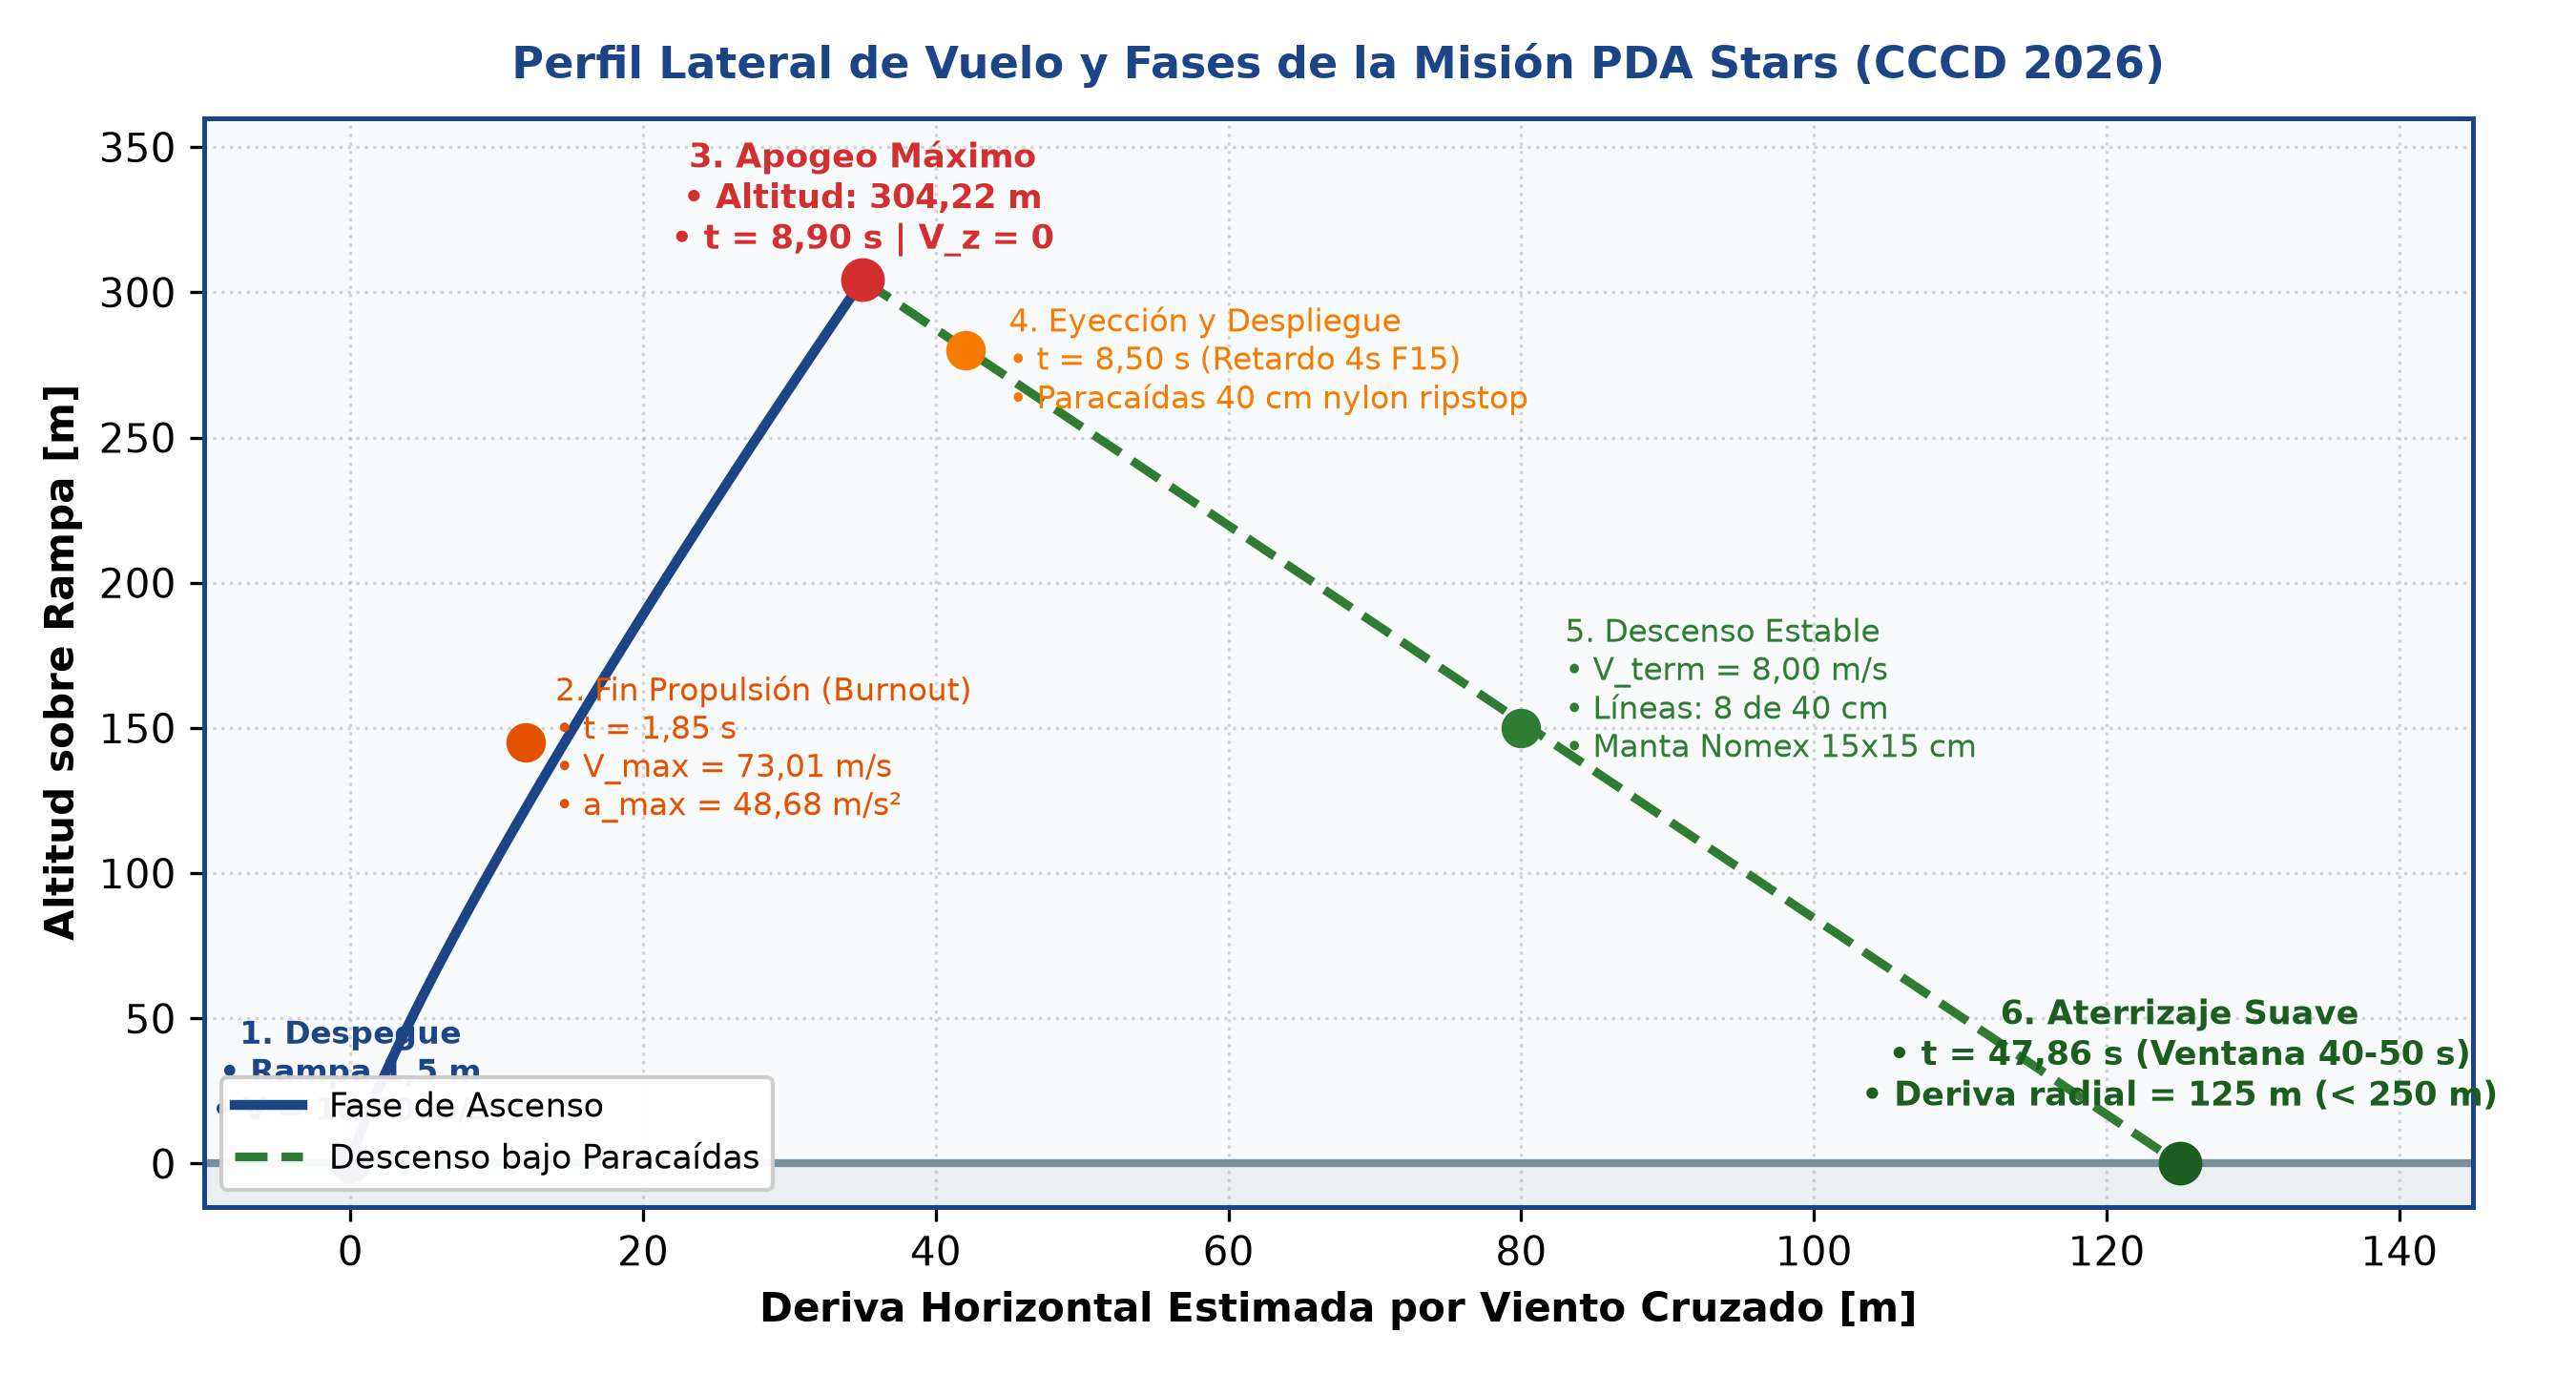
\includegraphics[width=0.95\linewidth]{fig_perfil_lateral_vuelo.png}
\caption{Perfil lateral de vuelo y eventos secuenciales de la misión PDA STARS.}
\label{fig:perfil_vuelo}
\end{figure}

\subsection{Curvas Dinámicas de Trayectoria}
A continuación se presentan las curvas temporales de altitud, velocidad y aceleración obtenidas del modelo validado:

\begin{figure}[H]
\centering
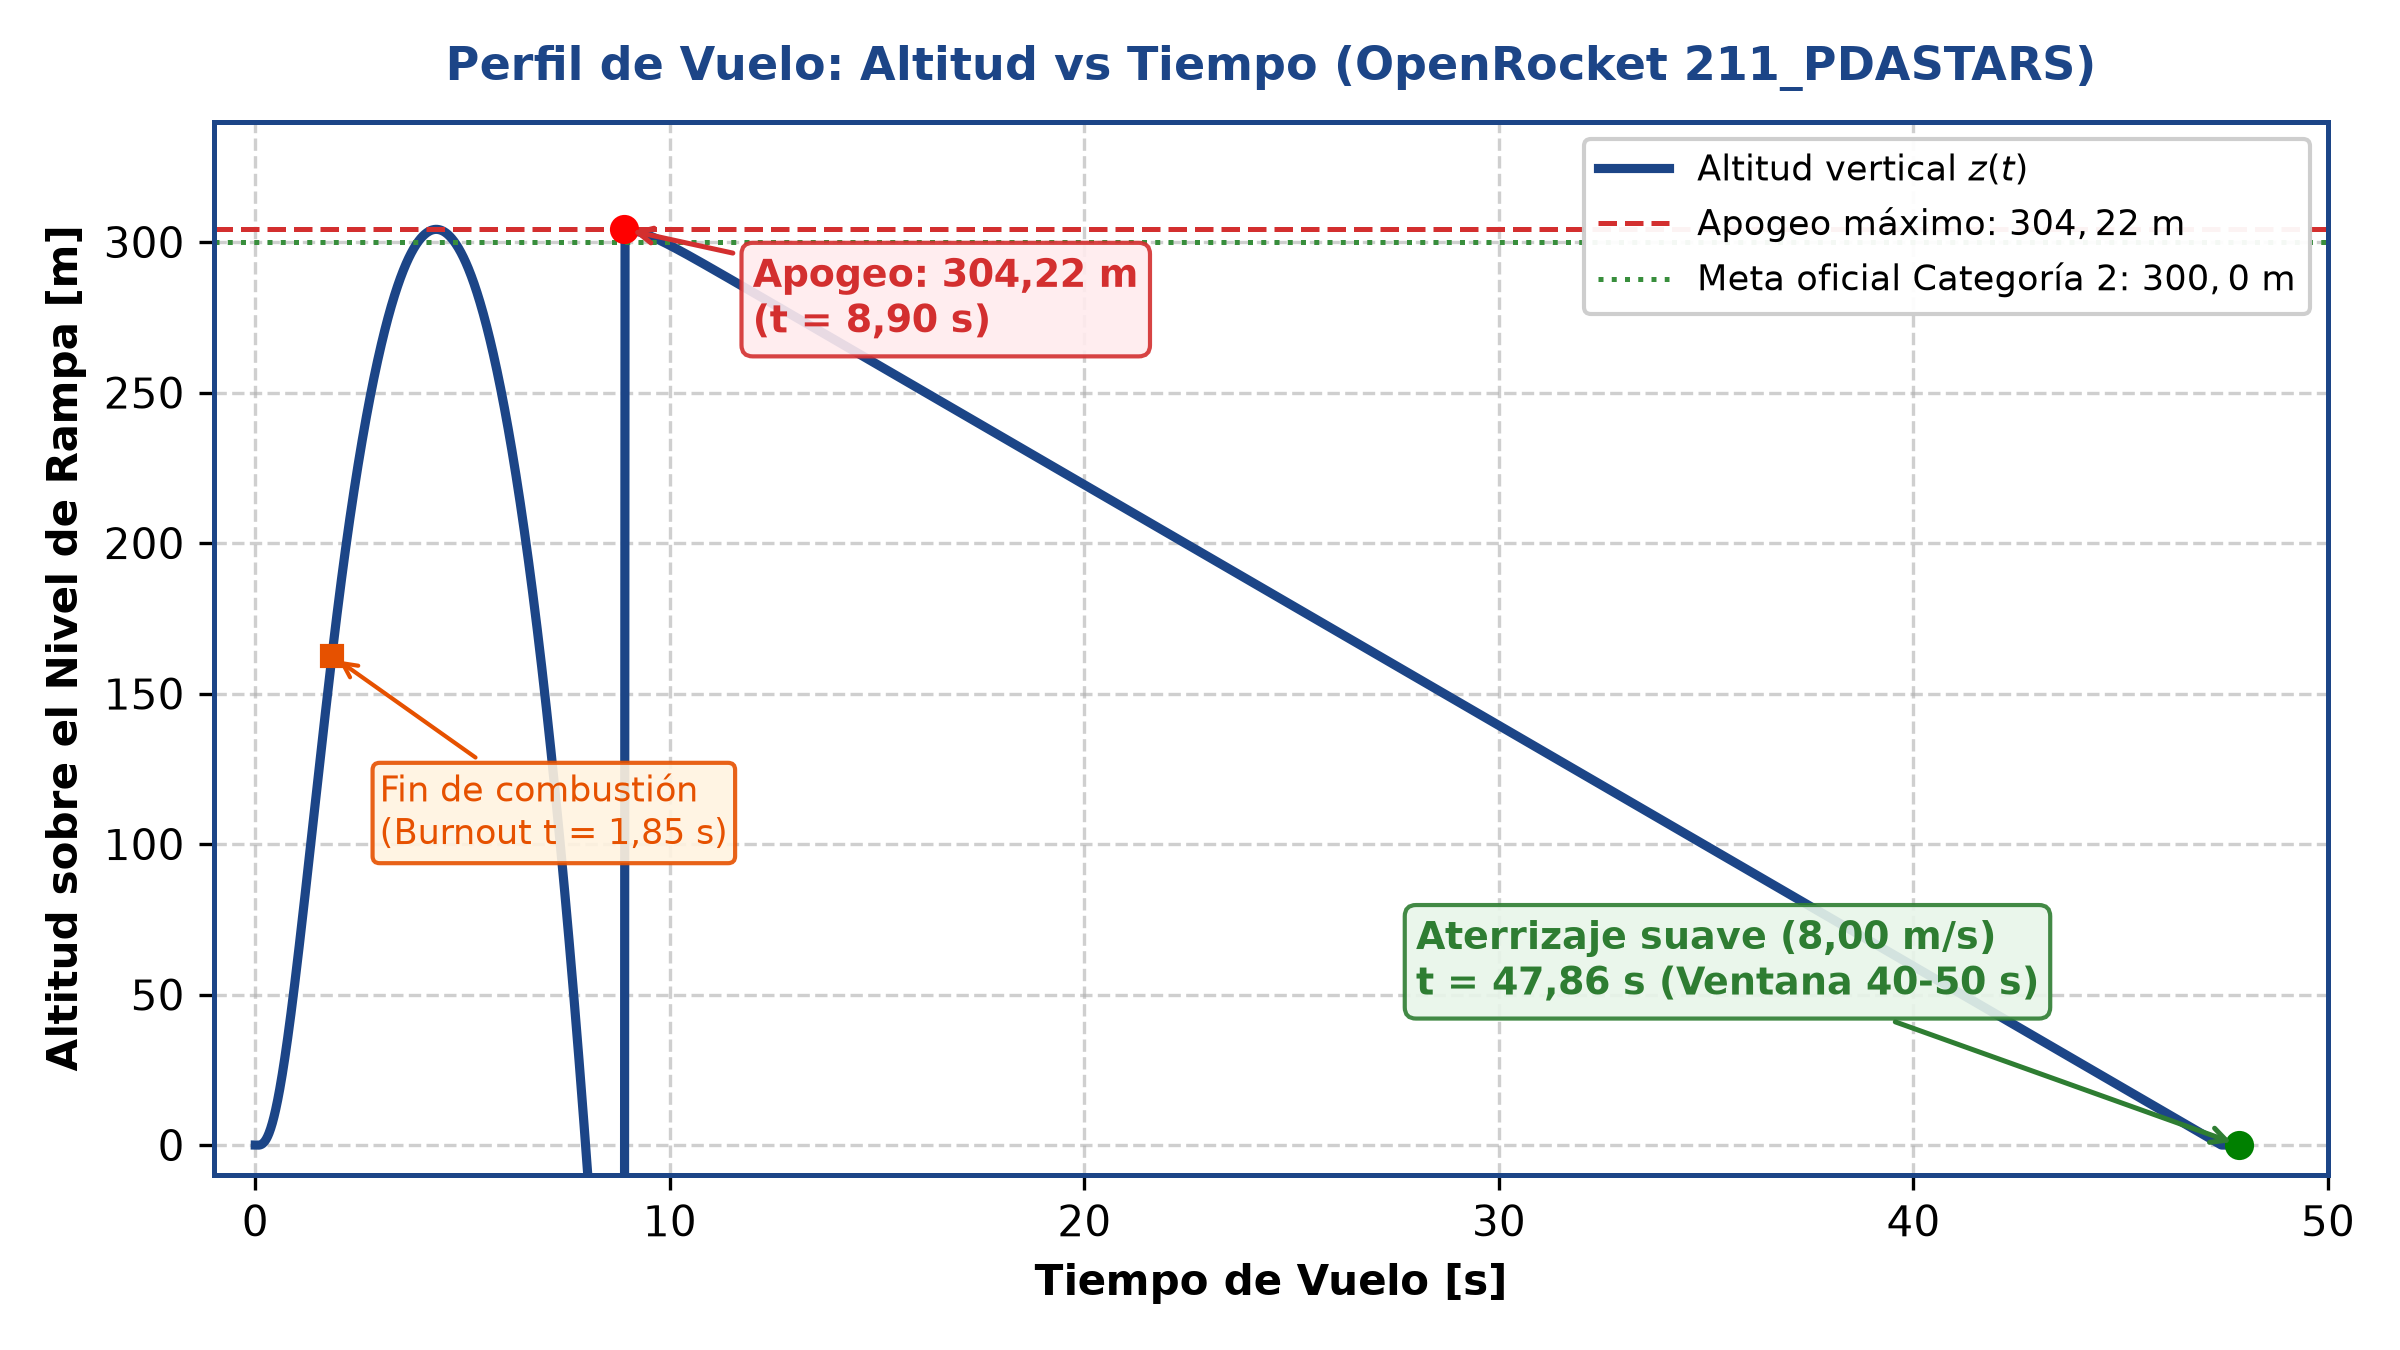
\includegraphics[width=0.9\linewidth]{fig_altitud_tiempo.png}
\caption{Curva de altitud vs tiempo (Apogeo máximo de $304,22\text{ m}$ y tiempo total de $47,86\text{ s}$).}
\label{fig:altitud_tiempo}
\end{figure}

\begin{figure}[H]
\centering
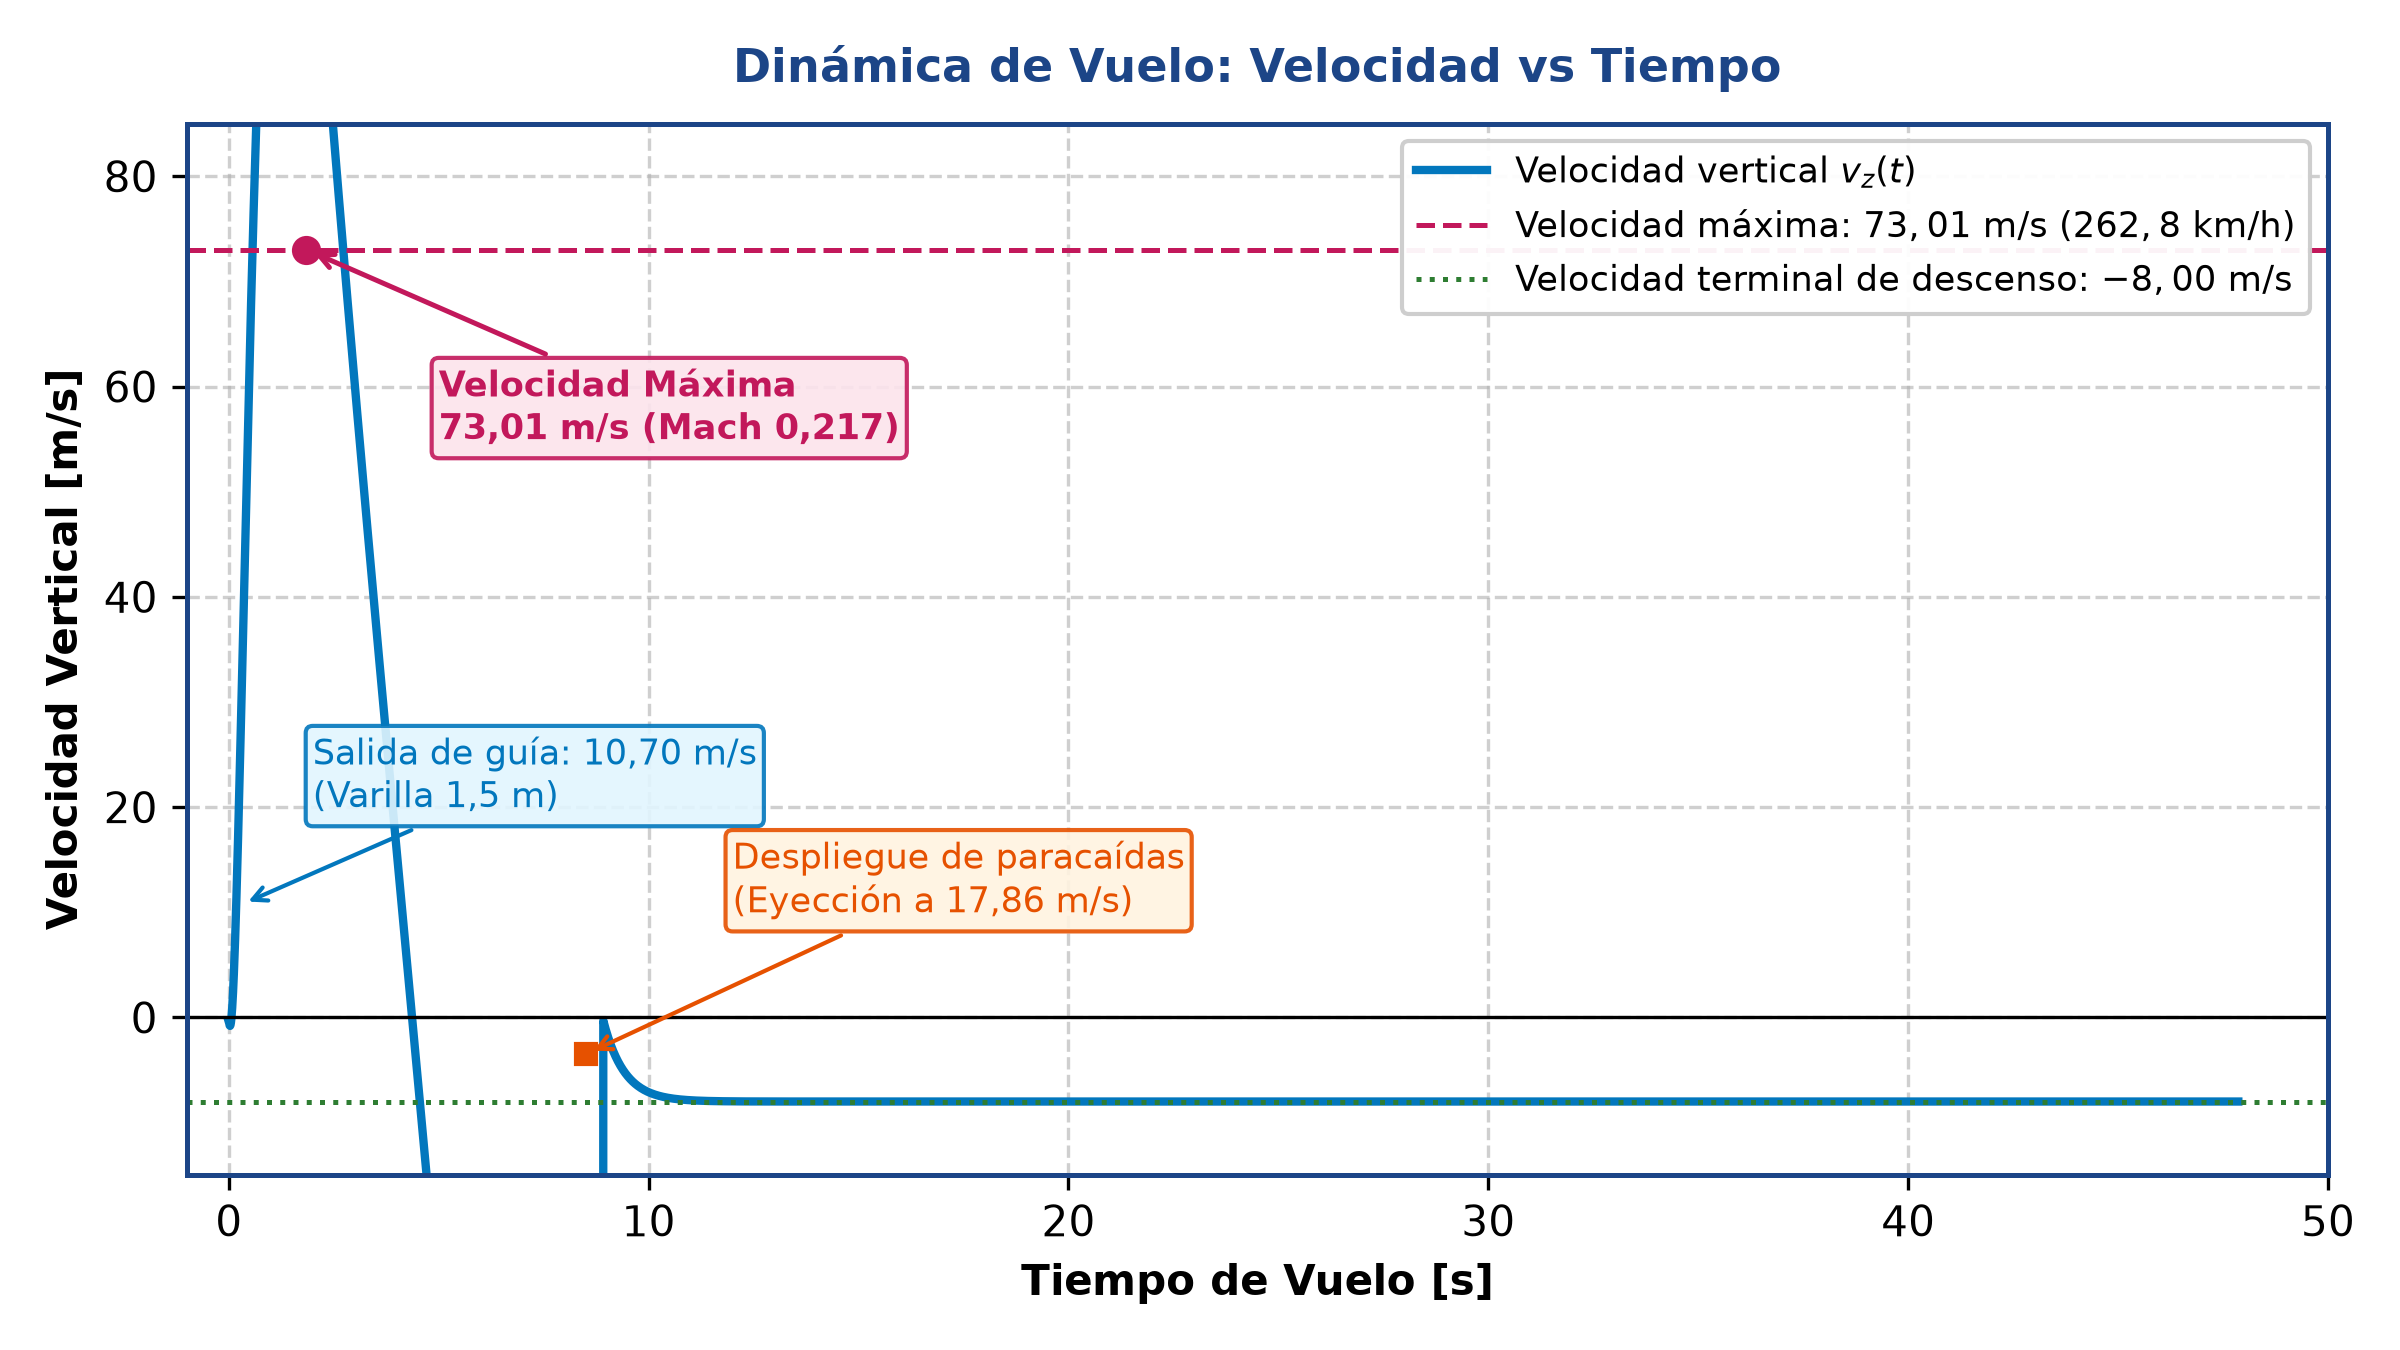
\includegraphics[width=0.9\linewidth]{fig_velocidad_tiempo.png}
\caption{Curva de velocidad vertical vs tiempo ($v_{max} = 73,01\text{ m/s}$, $v_{term} = 8,00\text{ m/s}$).}
\label{fig:velocidad_tiempo}
\end{figure}

\begin{figure}[H]
\centering
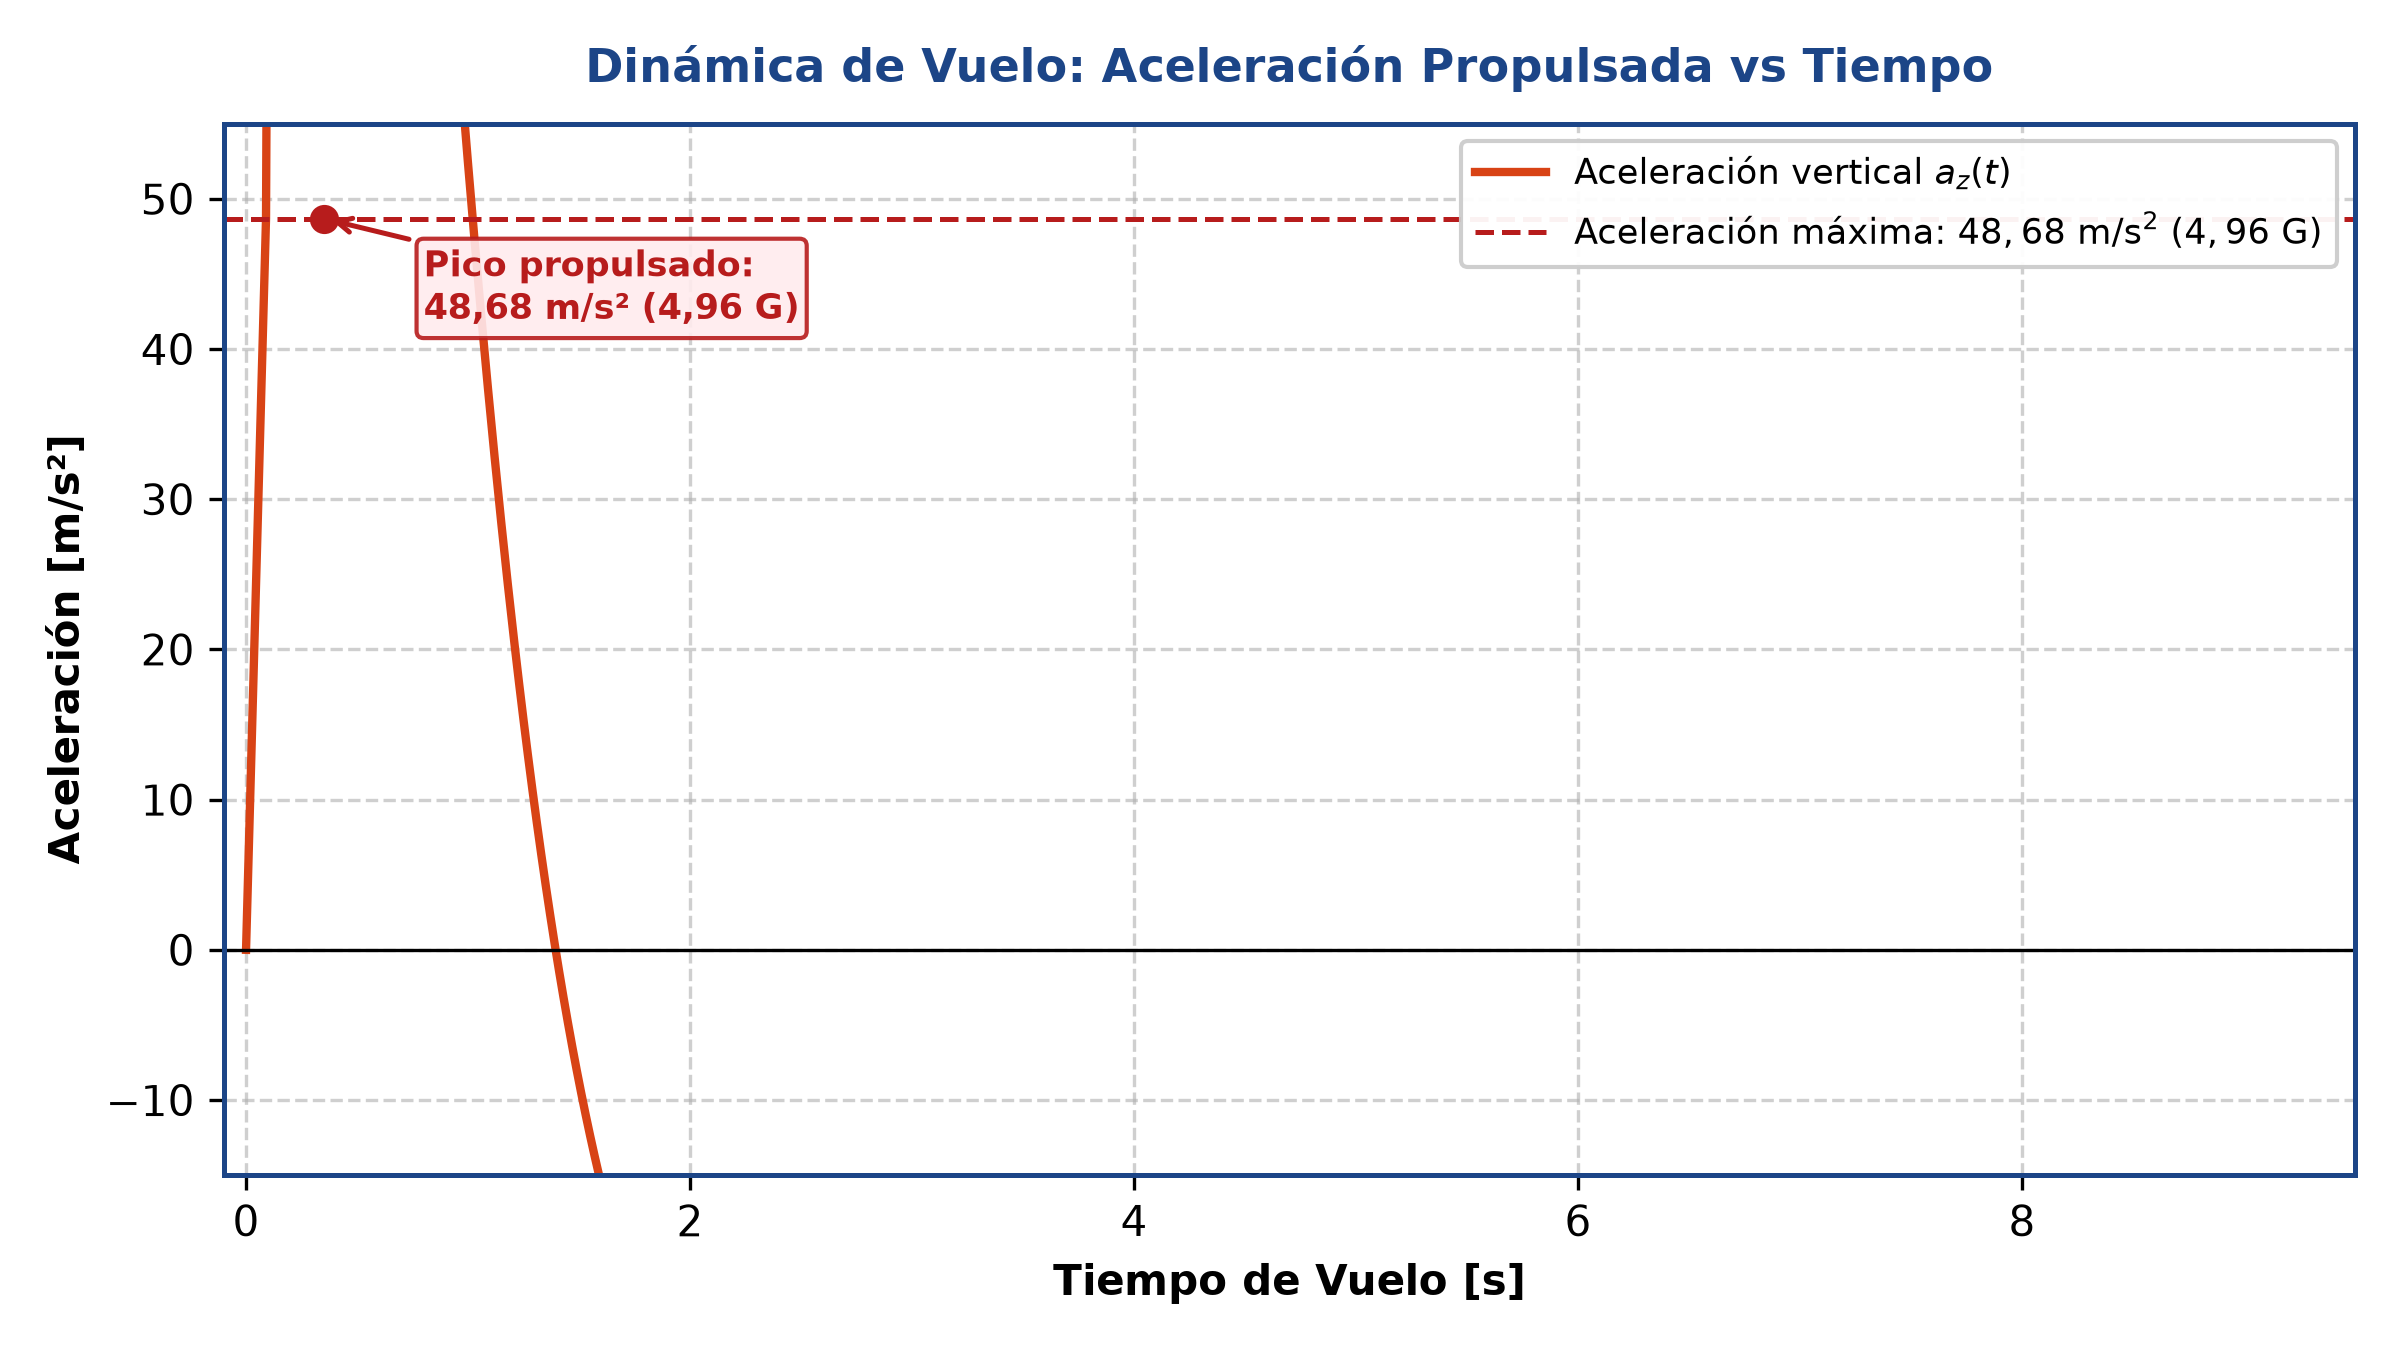
\includegraphics[width=0.9\linewidth]{fig_aceleracion_tiempo.png}
\caption{Curva de aceleración propulsada vs tiempo (pico máximo de $48,68\text{ m/s}^2$ / $4,96\text{ G}$).}
\label{fig:aceleracion_tiempo}
\end{figure}


% 7. CONSTRUCCIÓN Y MANUFACTURA
\section{Construcción y Manufactura}

La fabricación del cohete PDA STARS se basó en una estrategia híbrida que combina la ligereza del tubo Kraft enrollado en espiral con la precisión dimensional y rigidez mecánica de la manufactura aditiva FDM en filamentos de ingeniería.

\subsection{Diseño y Planificación de la Construcción}
Se generó el despiece computacional a partir de los modelos validados en OpenRocket y Fusion 360, estableciendo tolerancias de ajuste deslizante suave ($0,15\text{ -- }0,20\text{ mm}$) en la unión de la ojiva y la bahía de carga útil para evitar tanto el desacople prematuro por vibración como el bloqueo durante la sobrepresión de eyección.

\begin{figure}[H]
\centering
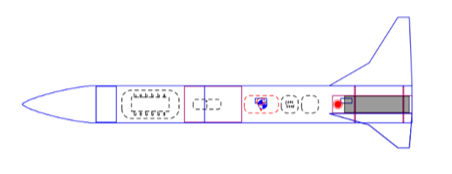
\includegraphics[width=0.85\linewidth]{diseno_openrocket.png}
\caption{Modelo geométrico y esquema de distribución interna en OpenRocket.}
\label{fig:openrocket_layout}
\end{figure}

\subsection{Modelado 3D de Componentes Estructurales}
Las aletas, anillos de centrado y acoples fueron diseñados con ranuras pasantes a través del fuselaje (\textit{through-the-wall}) para crear una unión monolítica entre el fuselaje Kraft y el tubo portamotor concéntrico de 29 mm.

\begin{figure}[H]
\centering
\begin{subfigure}[b]{0.45\linewidth}
    \centering
    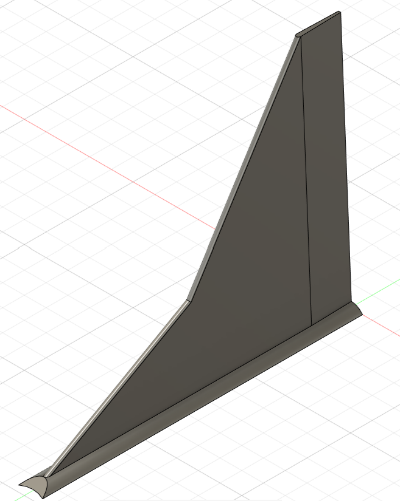
\includegraphics[height=3.5cm,keepaspectratio]{cad_aleta.png}
    \caption{Aleta en PETG-CF.}
\end{subfigure}
\hfill
\begin{subfigure}[b]{0.45\linewidth}
    \centering
    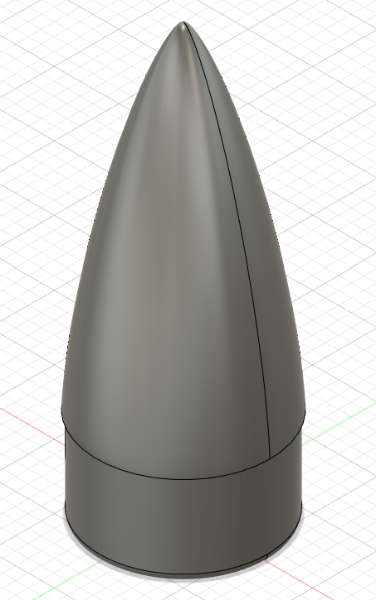
\includegraphics[height=3.5cm,keepaspectratio]{cad_ojiva.png}
    \caption{Ojiva Haack.}
\end{subfigure}
\vspace{0.3cm}
\begin{subfigure}[b]{0.45\linewidth}
    \centering
    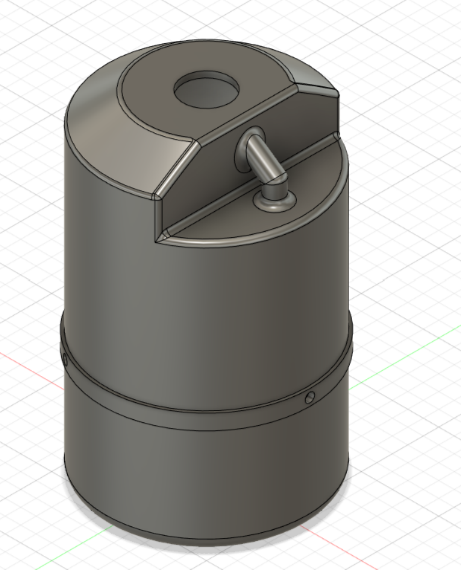
\includegraphics[height=3.5cm,keepaspectratio]{cad_acople.png}
    \caption{Acople con ojal.}
\end{subfigure}
\hfill
\begin{subfigure}[b]{0.45\linewidth}
    \centering
    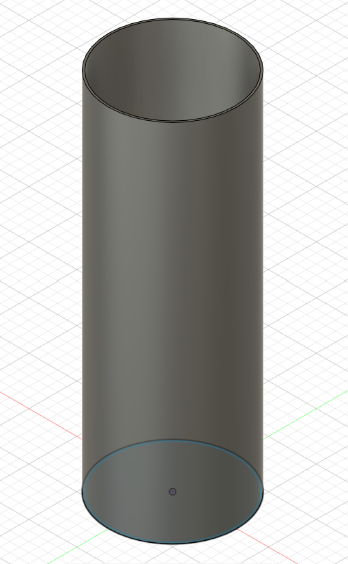
\includegraphics[height=3.5cm,keepaspectratio]{cad_centrador.png}
    \caption{Anillo de centrado.}
\end{subfigure}
\caption{Componentes modelados en CAD para manufactura aditiva FDM.}
\label{fig:cad_piezas}
\end{figure}

\subsection{Selección de Materiales y Criterio Técnico}
\begin{figure}[H]
\centering
\begin{subfigure}[b]{0.48\linewidth}
    \centering
    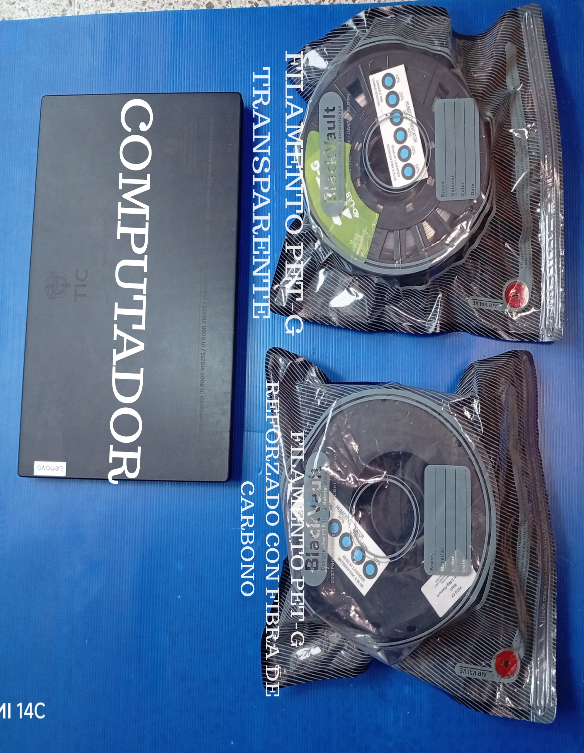
\includegraphics[height=4.5cm,keepaspectratio]{filamentos.png}
    \caption{Filamentos técnicos PETG y PETG-CF.}
\end{subfigure}
\hfill
\begin{subfigure}[b]{0.48\linewidth}
    \centering
    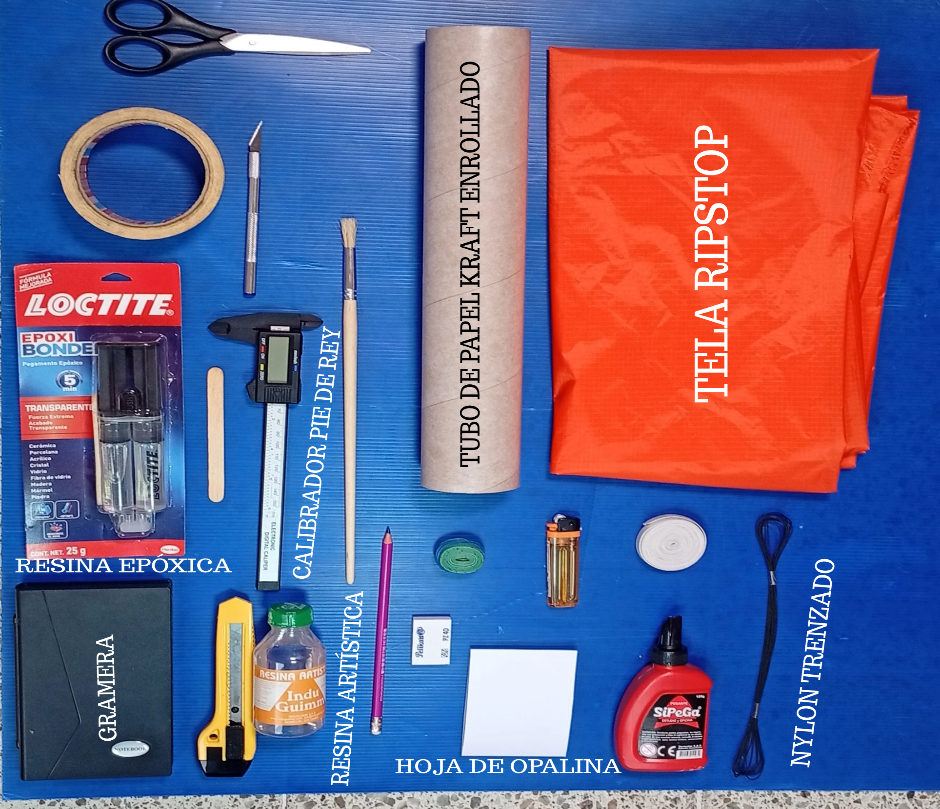
\includegraphics[height=4.5cm,keepaspectratio]{materiales.png}
    \caption{Materiales compuestos, epoxi y fuselaje.}
\end{subfigure}
\caption{Materiales seleccionados para la construcción de PDA STARS.}
\label{fig:materiales_utilizados}
\end{figure}

\begin{itemize}[leftmargin=1.5em]
    \item \textbf{PETG Estándar (Ojiva):} Empleado en la ojiva y carcasa de la carga útil para garantizar \textbf{permeabilidad electromagnética total} y evitar el efecto jaula de Faraday sobre las lecturas y antenas de telemetría.
    \item \textbf{PETG Reforzado con Fibra de Carbono (PETG-CF):} Utilizado exclusivamente en aletas y anillos de centrado por su módulo de elasticidad superior ($> 4,5\text{ GPa}$) y resistencia térmica ante gases de escape del motor F15.
    \item \textbf{Tubo Kraft Fenólico BT-80:} Ofrece alta resistencia específica a compresión y flexión con masa volumétrica reducida frente a tubos plásticos comerciales.
\end{itemize}

\subsection{Proceso de Fabricación y Ensamble}
\begin{figure}[H]
\centering
\begin{subfigure}[b]{0.48\linewidth}
    \centering
    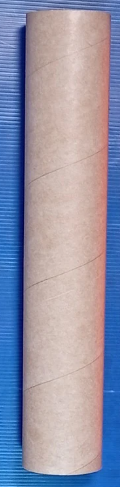
\includegraphics[height=4.2cm,keepaspectratio]{tubo_recibido.png}
    \caption{Corte y calibración de tubos Kraft BT-80.}
\end{subfigure}
\hfill
\begin{subfigure}[b]{0.48\linewidth}
    \centering
    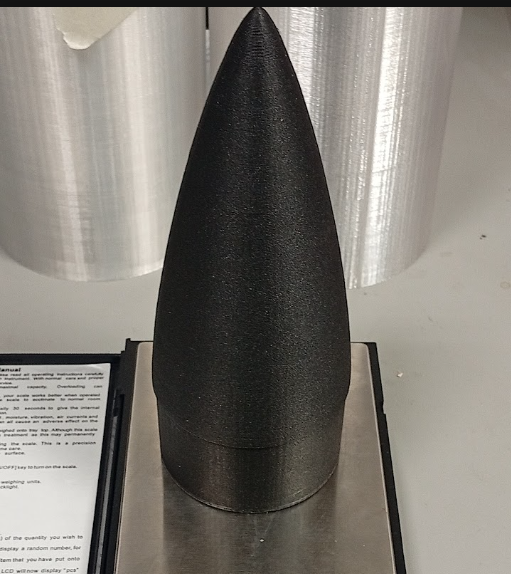
\includegraphics[height=4.2cm,keepaspectratio]{ojiva_impresa.png}
    \caption{Ojiva impresa en PETG con acabado pulido.}
\end{subfigure}
\caption{Mecanizado de fuselaje y manufactura aditiva de la ojiva.}
\label{fig:fabricacion_piezas}
\end{figure}

\begin{figure}[H]
\centering
\begin{subfigure}[b]{0.48\linewidth}
    \centering
    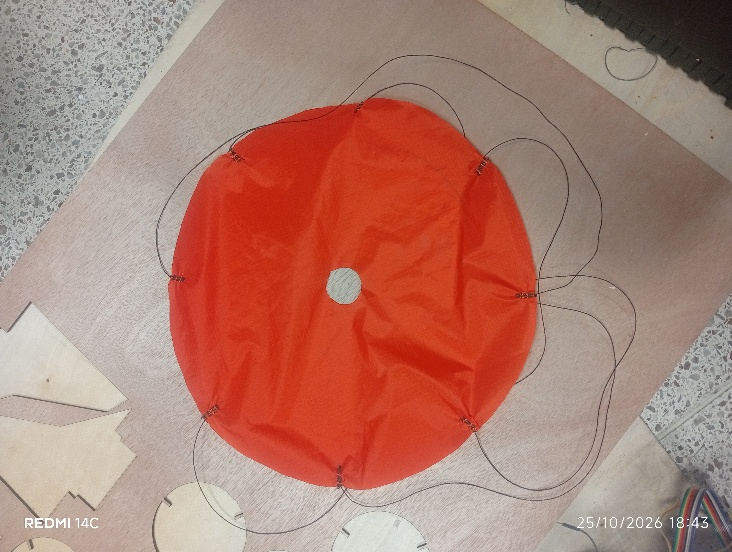
\includegraphics[height=4.2cm,keepaspectratio]{paracaidas_fisico.jpg}
    \caption{Paracaídas de 40 cm en tela ripstop con 8 líneas.}
\end{subfigure}
\hfill
\begin{subfigure}[b]{0.48\linewidth}
    \centering
    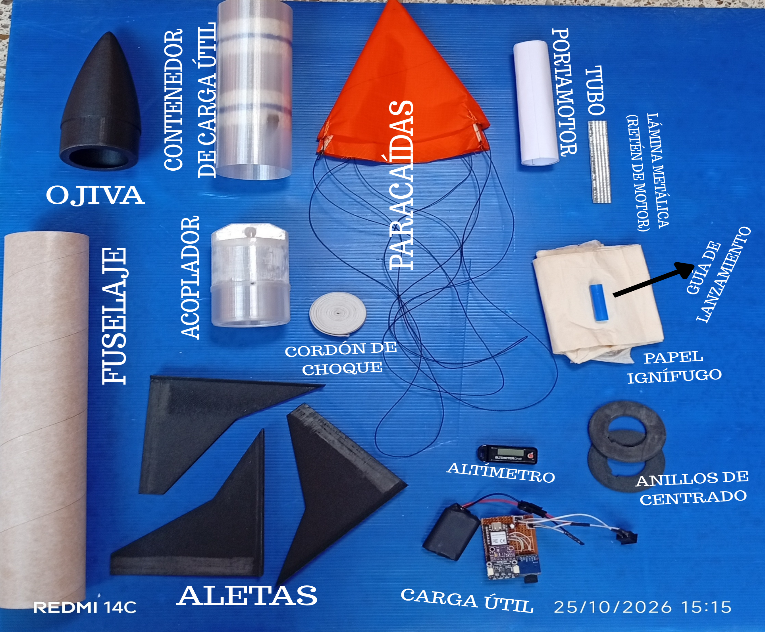
\includegraphics[height=4.2cm,keepaspectratio]{partes_sin_ensamblar.png}
    \caption{Inspección previa de componentes físicos listos.}
\end{subfigure}
\caption{Sistema de recuperación y verificación previa al ensamble estructural.}
\label{fig:componentes_previos}
\end{figure}

\begin{figure}[H]
\centering
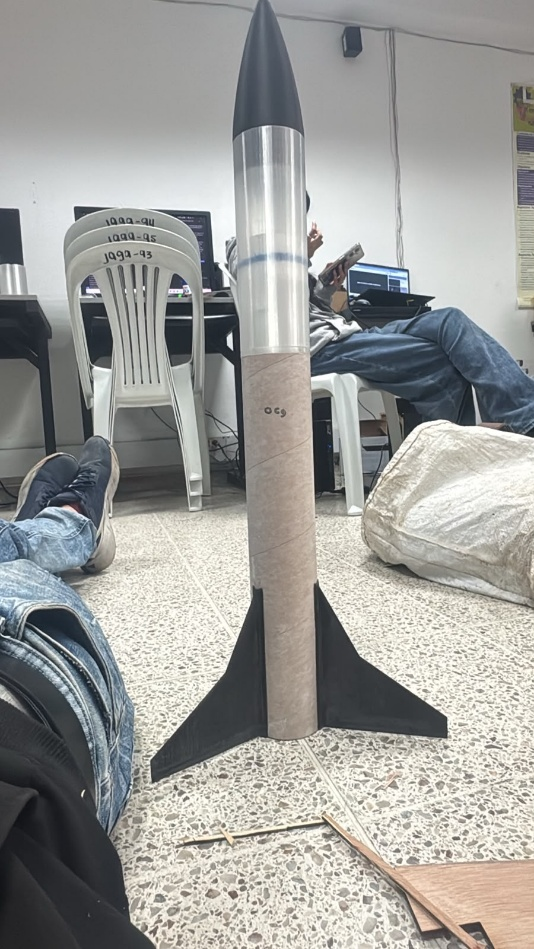
\includegraphics[height=7.0cm,keepaspectratio]{cohete_terminado.jpg}
\caption{Cohete PDA STARS completamente ensamblado en taller.}
\label{fig:cohete_terminado}
\end{figure}

\subsection{Balance de Masas Final}
\begin{table}[H]
\centering
\small
\begin{tabularx}{\linewidth}{Xccc}
\toprule
\rowcolor{navyiejaga!15}
\textbf{Subconjunto / Componente} & \textbf{Masa Teórica (ORK)} & \textbf{Masa Real Taller} & \textbf{Desviación} \\
\midrule
Ojiva Haack PETG & 39,7 g & 41,2 g & $+3,8\%$ \\
\rowcolor{grisclaro}
Bahía y contenedor de carga útil & 60,0 g & 60,0 g & $0,0\%$ (Cumple $\le 60\text{ g}$) \\
Instrumentación electrónica y batería & 9,9 g & 10,5 g & $+6,0\%$ \\
\rowcolor{grisclaro}
Fuselaje principal Kraft BT-80 & 30,0 g & 31,4 g & $+4,6\%$ \\
Conjunto de 3 aletas en PETG-CF & 64,0 g & 63,8 g & $-0,3\%$ \\
\rowcolor{grisclaro}
Portamotor 29 mm y centradores & 14,0 g & 14,6 g & $+4,2\%$ \\
Paracaídas 40 cm, manta Nomex y Kevlar & 11,0 g & 11,5 g & $+4,5\%$ \\
\rowcolor{grisclaro}
Adhesivo epóxico y acabados & 53,5 g & 54,0 g & $+0,9\%$ \\
\midrule
\textbf{Masa total en seco (Dry Mass)} & \textbf{282,1 g} & \textbf{287,0 g} & $+1,7\%$ \\
\rowcolor{grisclaro}
Motor Estes F15-4 cargado & 91,0 g & 91,0 g & $0,0\%$ \\
Instrumentación complementaria en rampa & 150,0 g & 150,0 g & $0,0\%$ \\
\midrule
\rowcolor{navyiejaga!10}
\textbf{Masa total en rampa (Liftoff Mass)} & \textbf{523,1 g} & \textbf{528,0 g} & $\mathbf{+0,9\%}$ (Límite $< 650\text{ g}$) \\
\bottomrule
\end{tabularx}
\caption{Balance de masas estimado vs medido en báscula digital de precisión.}
\label{tab:balance_masas}
\end{table}


% 8. PARACAÍDAS Y SISTEMA DE RECUPERACIÓN
\section{Paracaídas y Sistema de Recuperación}

El sistema de recuperación del cohete PDA STARS tiene como función primordial desacelerar el vehículo desde el apogeo ($304,22\text{ m}$) hasta la superficie con una velocidad terminal nominal de \textbf{8,00 m/s}, permitiendo que la estructura aterrice sin daño alguno y asegurando que la duración total del vuelo se sitúe estrictamente dentro de la ventana reglamentaria de \textbf{40 a 50 segundos} para motores de clase F.

\subsection{Dimensionamiento Aerodinámico del Paracaídas}
El paracaídas consiste en un domo hemisférico de \textbf{40 cm de diámetro} ($D_p = 0,40\text{ m}$) confeccionado en tela ripstop nylon ripstop de 40 g/m² con baja porosidad, provisto de \textbf{ocho líneas de suspensión} de cuerda de nylon trenzado de 40 cm de longitud ancladas uniformemente en la periferia.

El área de referencia proyectada es:
\begin{equation}
    S_p = \frac{\pi D_p^2}{4} = \frac{\pi (0,40)^2}{4} \approx 0,1257\text{ m}^2
\end{equation}
Para una masa total en descenso de $m = 437\text{ g}$ ($0,437\text{ kg}$, tras la expulsión de propelente), una densidad atmosférica local $\rho = 1,05\text{ kg/m}^3$ y un coeficiente de arrastre experimental del paracaídas hemisférico $C_d = 0,78$, la velocidad terminal de descenso en equilibrio cuasi-estático es:
\begin{equation}
    v_{\text{term}} = \sqrt{\frac{2 m g}{\rho S_p C_d}} = \sqrt{\frac{2 \cdot 0,437 \cdot 9,81}{1,05 \cdot 0,1257 \cdot 0,78}} \approx \mathbf{8,00\text{ m/s}}
\end{equation}
Este valor coincide con una precisión de dos decimales con la simulación numérica oficial de OpenRocket ($7,998\text{ m/s}$ en \texttt{simulacion\_stellaris.csv}), lo que arroja un tiempo de descenso en paracaídas de:
\begin{equation}
    t_{\text{descenso}} = \frac{304,22\text{ m}}{8,00\text{ m/s}} \approx 38,0\text{ s}
\end{equation}
Sumado al tiempo de ascenso hasta el apogeo ($8,90\text{ s}$), el tiempo total de vuelo resulta en:
\begin{equation}
    t_{\text{total}} = 8,90\text{ s} + 38,0\text{ s} \approx \mathbf{47,86\text{ segundos}}
\end{equation}
posicionando al cohete en el centro de la ventana oficial de 40 a 50 segundos.

\subsection{Cálculo de Deriva Radial por Viento Cruzado}
Considerando una capa de viento atmosférico lateral constante de $v_w = 3,5\text{ m/s}$ (condición máxima admisible en rampa según el manual de seguridad), la deriva horizontal teórica máxima $R$ es:
\begin{equation}
    R = v_w \cdot t_{\text{descenso}} = 3,5\text{ m/s} \cdot 38,0\text{ s} \approx 133\text{ metros}
\end{equation}
Este radio proporciona un margen de seguridad de más de 117 metros respecto al límite de exclusión obligatorio de \textbf{250 metros} fijado en la circular oficial de Zonas de Recuperación del CCCD 2026.

\subsection{Diagrama del Tren de Recuperación y Protección Térmica}
Para evitar la separación accidental de módulos durante el shock de apertura (estimado en $8\text{ -- }10\text{ G}$ dinámicos), todos los elementos estructurales se encuentran unidos mecánicamente en un tren continuo mediante un cordón tubular de Kevlar ignífugo de \textbf{3,6 metros} (12 pies) de longitud:
\begin{itemize}[leftmargin=1.5em]
    \item \textbf{Punto 1 (Extremo Superior):} Sujeción a la ojiva mediante cáncamo roscado M4.
    \item \textbf{Punto 2 (Cuerpo Intermedio):} Fijación al ojal estructural integrado en la base de la bahía de carga útil (ensayado a tracción de 250 N), asegurando que la carga útil permanezca solidaria al cohete en todo momento conforme a la Sección 5 de la Guía de Carga Útil.
    \item \textbf{Punto 3 (Arnés del Paracaídas):} Vínculo a las 8 líneas de suspensión mediante nudo de ocho por seno y eslabón rápido.
    \item \textbf{Punto 4 (Extremo Inferior):} Anclaje al anillo de centrado superior de la bahía motriz.
\end{itemize}

\begin{figure}[H]
\centering
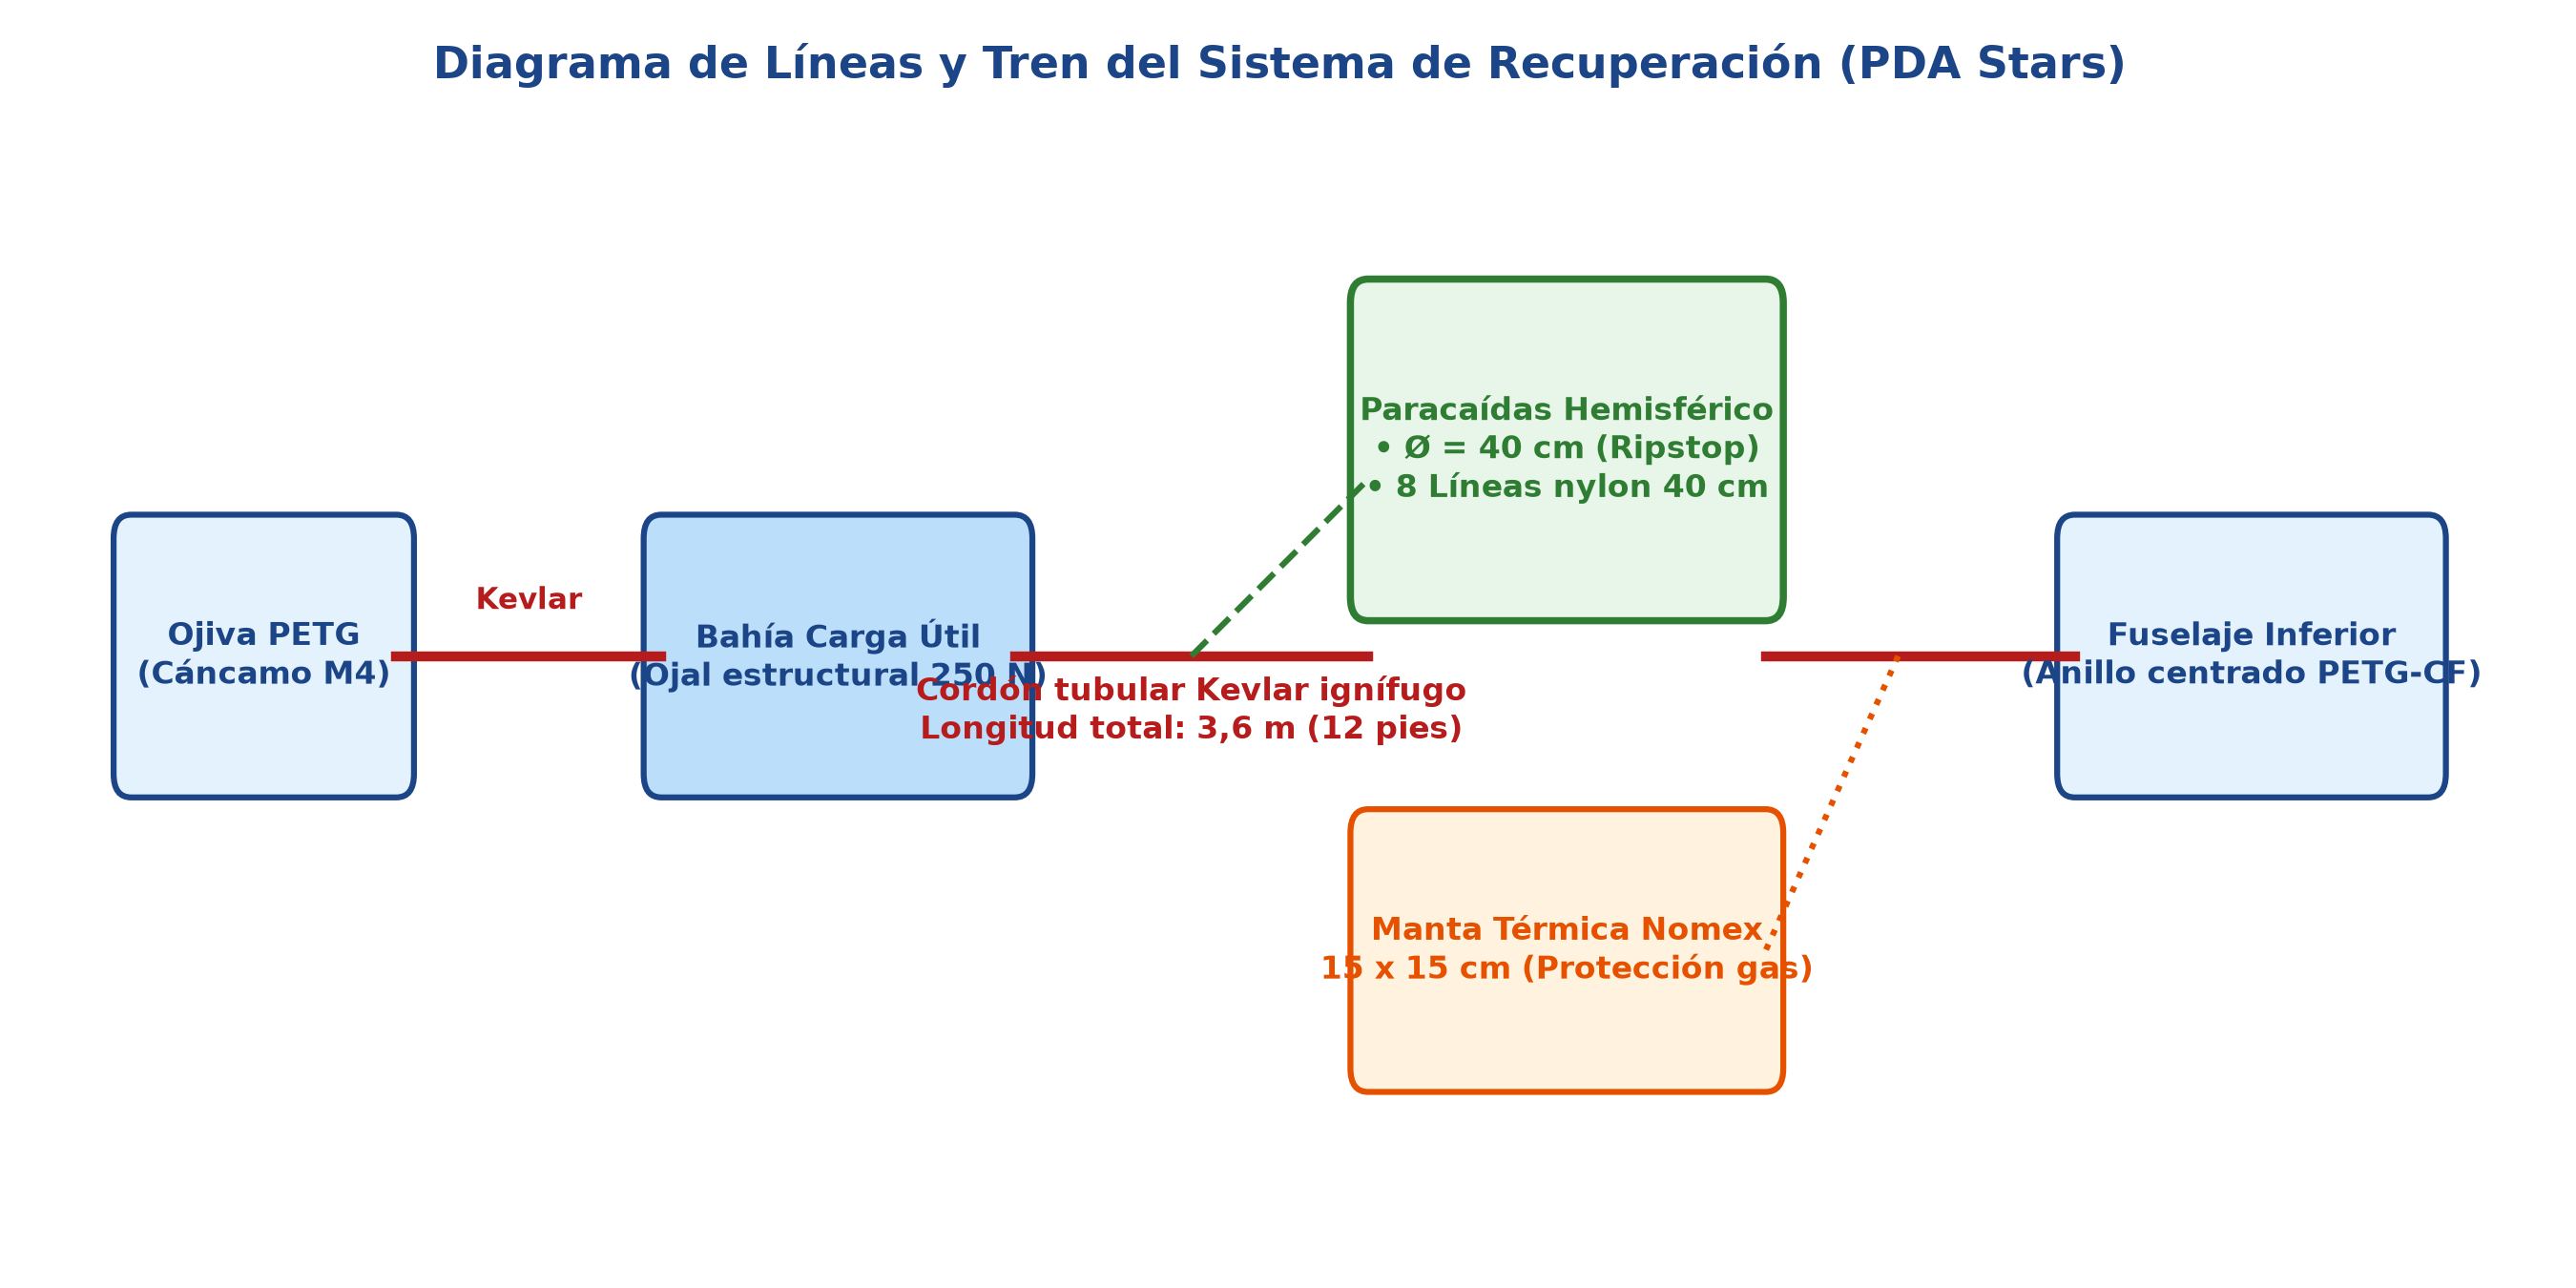
\includegraphics[width=0.92\linewidth]{fig_diagrama_lineas_recuperacion.png}
\caption{Diagrama esquemático de líneas y amarres del tren de recuperación de PDA STARS.}
\label{fig:diagrama_recuperacion}
\end{figure}

Para salvaguardar la tela de ripstop y las cuerdas de nylon del choque térmico generado por la carga de eyección de pólvora negra del motor F15-4 (retardo de 4 s), se intercala una \textbf{manta de protección térmica Nomex de 15x15 cm} (masa de 3,0 g) impregnada y doblada en acordeón sobre el tubo portamotor, sustituyendo por completo la necesidad de wadding desechable.


% 9. CARGA ÚTIL
\section{Carga Útil}

La carga útil experimental de PDA STARS consiste en una unidad autónoma de telemetría e instrumentación aeroespacial diseñada para registrar las variables termodinámicas y cinemáticas del vuelo, procesarlas en tiempo real y salvaguardar los registros científicos. Su masa total es de exactamente \textbf{60,0 gramos}, dando cumplimiento estricto a la restricción reglamentaria de $\le 60\text{ g}$.

\subsection*{Propósito del experimento}
La carga útil de nuestro cohete es un sistema de medición compacto que vuela dentro del vehículo para registrar datos de vuelo en tiempo real. Su objetivo es medir la altitud alcanzada, la velocidad, la aceleración y detectar automáticamente en qué fase del vuelo se encuentra el cohete (reposo en rampa, ascenso propulsado, trayectoria libre, apogeo, descenso bajo paracaídas y aterrizaje). Esto permite comparar lo que predijo la simulación en OpenRocket con lo que realmente ocurrió durante el lanzamiento.

\subsection*{Principio de funcionamiento}
El sistema opera con un microcontrolador \textbf{Seeeduino XIAO} (arquitectura ARM Cortex-M0+ a 48 MHz), una placa pequeña, ligera y de bajo consumo. Dispone de dos sensores principales:
\begin{itemize}[leftmargin=1.5em]
    \item Un barómetro digital de alta precisión \textbf{DPS310}, que mide la presión ambiental y calcula la altitud relativa con resolución sub-métrica (hasta $\pm 0,05\text{ m}$).
    \item Un sensor inercial \textbf{MPU6050}, que mide las aceleraciones y velocidades angulares en tres ejes espaciales ($X, Y, Z$).
\end{itemize}
Los sensores se comunican con el microcontrolador mediante bus digital I2C. Los datos se almacenan cada 50 milisegundos (tasa de muestreo de 20 Hz) en una memoria microSD.

\subsection*{Procesamiento de los datos}
Como las señales de los sensores presentan fluctuaciones y ruido electromagnético natural, se implementaron dos filtros digitales en el firmware:
\begin{itemize}[leftmargin=1.5em]
    \item Un \textbf{filtro pasa-bajas} para el sensor inercial, el cual elimina las vibraciones mecánicas generadas por la combustión del motor y la resistencia aerodinámica.
    \item Un \textbf{filtro de Kalman} unidimensional que fusiona las lecturas de altitud barométrica del DPS310 con la aceleración vertical del MPU6050, produciendo una curva de trayectoria suave y altamente confiable.
\end{itemize}

\subsection*{Variables a estudiar y metodología}
Las variables registradas durante la misión son: presión estática, temperatura ambiental, altitud barométrica relativa, velocidad vertical calculada por integración y aceleraciones triaxiales. 

\subsection*{Calibración al encender}
Al energizarse en la rampa de lanzamiento, el sistema ejecuta una rutina automática de calibración durante aproximadamente 2 segundos mientras el cohete permanece inmóvil. En este lapso promedia 40 lecturas consecutivas de presión atmosférica para establecer el nivel cero de altitud sobre la rampa y calcula los offsets de gravedad en los acelerómetros.

\subsection*{Detección de las fases del vuelo}
El algoritmo de la máquina de estados reconoce automáticamente cada etapa del vuelo:
\begin{enumerate}[leftmargin=1.5em]
    \item \textbf{En rampa:} Espera hasta detectar una aceleración sostenida superior a $2,0\text{ G}$.
    \item \textbf{Ascenso:} Inicia el muestreo a máxima frecuencia y calcula la velocidad vertical.
    \item \textbf{Apogeo:} Identifica el instante en que la velocidad vertical cambia de signo (cruza por cero) y la altitud alcanza su punto de inflexión.
    \item \textbf{Descenso:} Monitorea que la velocidad de caída se estabilice en torno a los 8 m/s bajo paracaídas.
    \item \textbf{Aterrizaje:} Al detectar tres segundos continuos sin variación en altitud y aceleración cercana a 1 G, cierra ordenadamente el archivo de la tarjeta microSD y emite una señal sonora de localización.
\end{enumerate}

\subsection*{Componentes y conexiones}
A continuación se presenta el diagrama esquemático de interconexión eléctrica del sistema de aviónica:

\begin{figure}[H]
\centering
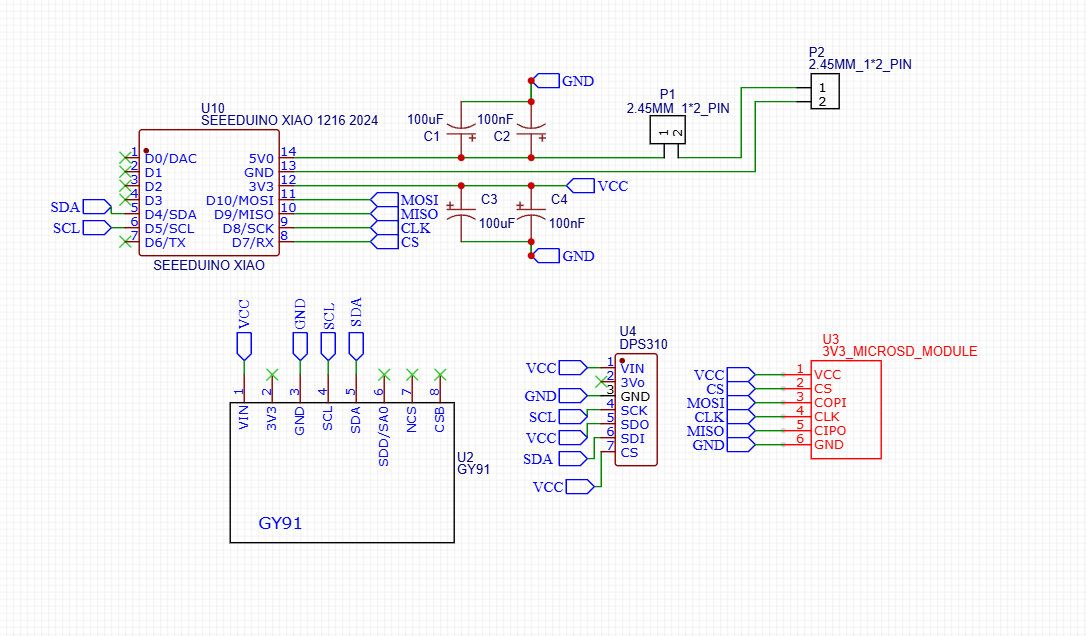
\includegraphics[width=0.8\linewidth]{esquematico_carga_util.png}
\caption{Diagrama esquemático de conexiones electrónicas de la carga útil.}
\label{fig:esquematico_payload}
\end{figure}

\subsection*{Montaje experimental}
El conexionado físico de los módulos y las pruebas preliminares de integración se realizaron inicialmente en placa de prototipado rápido para validar la integridad de las líneas de alimentación y bus I2C:

\begin{figure}[H]
\centering
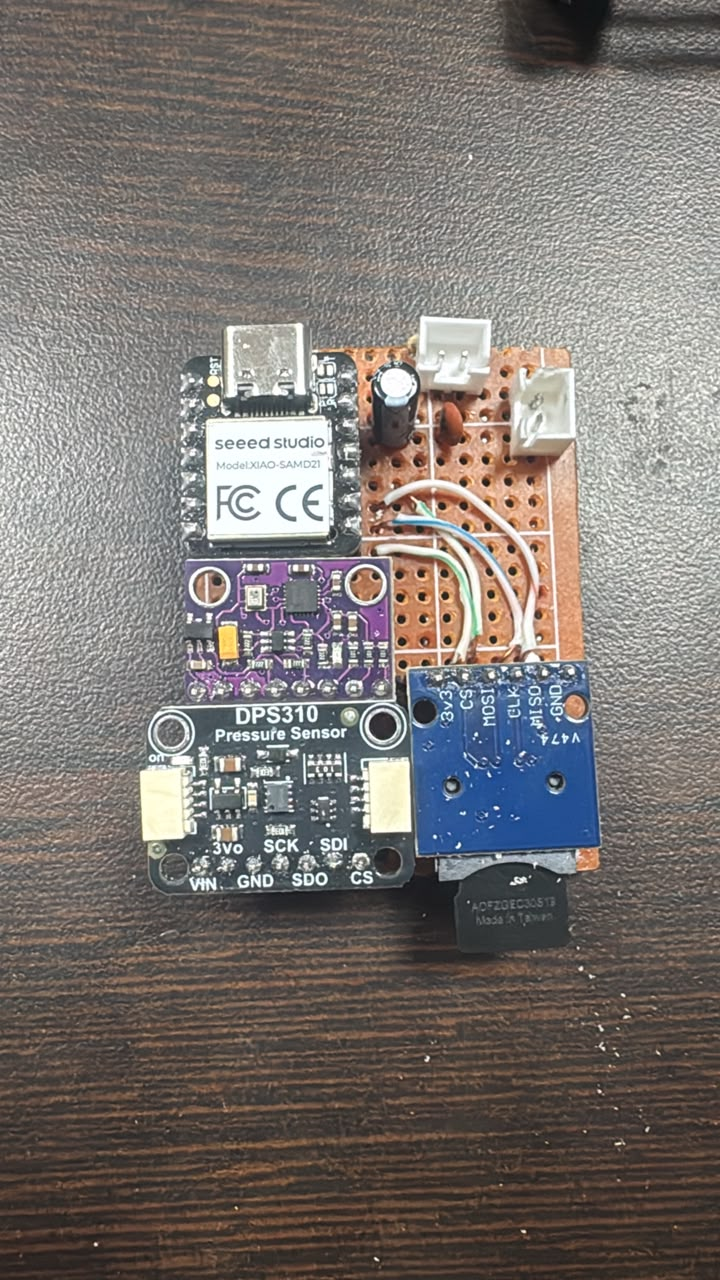
\includegraphics[width=0.75\linewidth]{montaje_experimental.jpg}
\caption{Montaje experimental físico y conexionado de la carga útil.}
\label{fig:montaje_payload}
\end{figure}

Para el vuelo final se desarrolló una placa de circuito impreso (PCB) fabricada mediante fresado CNC en placa de baquelita FR4, proporcionando alta rigidez y eliminando cables sueltos que pudieran desconectarse por choque dinámico:

\begin{figure}[H]
\centering
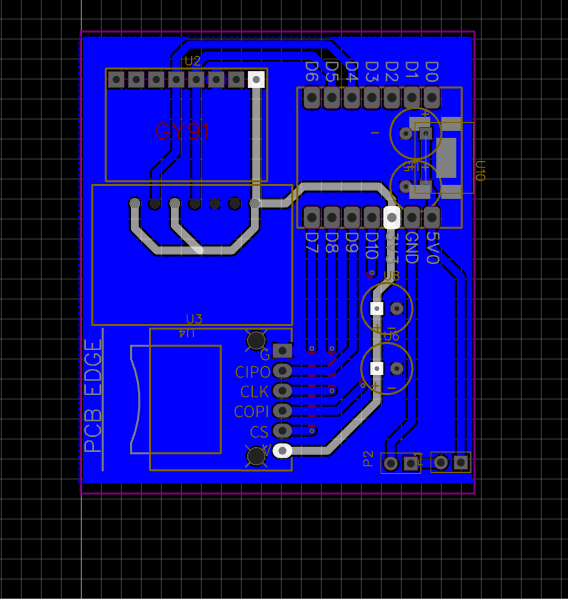
\includegraphics[width=0.75\linewidth]{pcb_carga_util.png}
\caption{Placa de circuito impreso (PCB) desarrollada para la carga útil.}
\label{fig:pcb_payload}
\end{figure}

\subsection*{Alimentación eléctrica}
El sistema se energiza mediante una batería recargable compacta de níquel-metal hidruro (NiMH) de \textbf{3,6 V y 150 mAh}, seleccionada por su estabilidad química ante variaciones de temperatura y nulo riesgo de inflamación frente a polímeros de litio. El consumo medio de corriente del conjunto (Seeeduino + sensores + micro-SD) es de aproximadamente 28 mA, garantizando una autonomía operativa superior a \textbf{3,5 horas}.

\subsection*{Respaldo de los datos principales}
Como salvaguarda ante una eventual falla mecánica o expulsión de la tarjeta microSD durante el shock de aterrizaje, las variables críticas del vuelo (altitud máxima en apogeo, velocidad máxima de ascenso, aceleración pico y tiempo total hasta el apogeo) se escriben directamente en la \textbf{memoria no volátil EEPROM} interna del microcontrolador al momento de detectarse el apogeo.

\subsection*{Telemetría y estación en tierra}
La carga útil de Categoría 2 opera bajo la modalidad de registro a bordo (\textit{data logger}), priorizando la confiabilidad y la ligereza del sistema. No obstante, para la lectura y análisis inmediato pos-vuelo en la zona de recuperación, se diseñó una interfaz gráfica desarrollada en Python (Tkinter/Matplotlib) que descarga los datos vía puerto serie USB y grafica instantáneamente la trayectoria:

\begin{figure}[H]
\centering
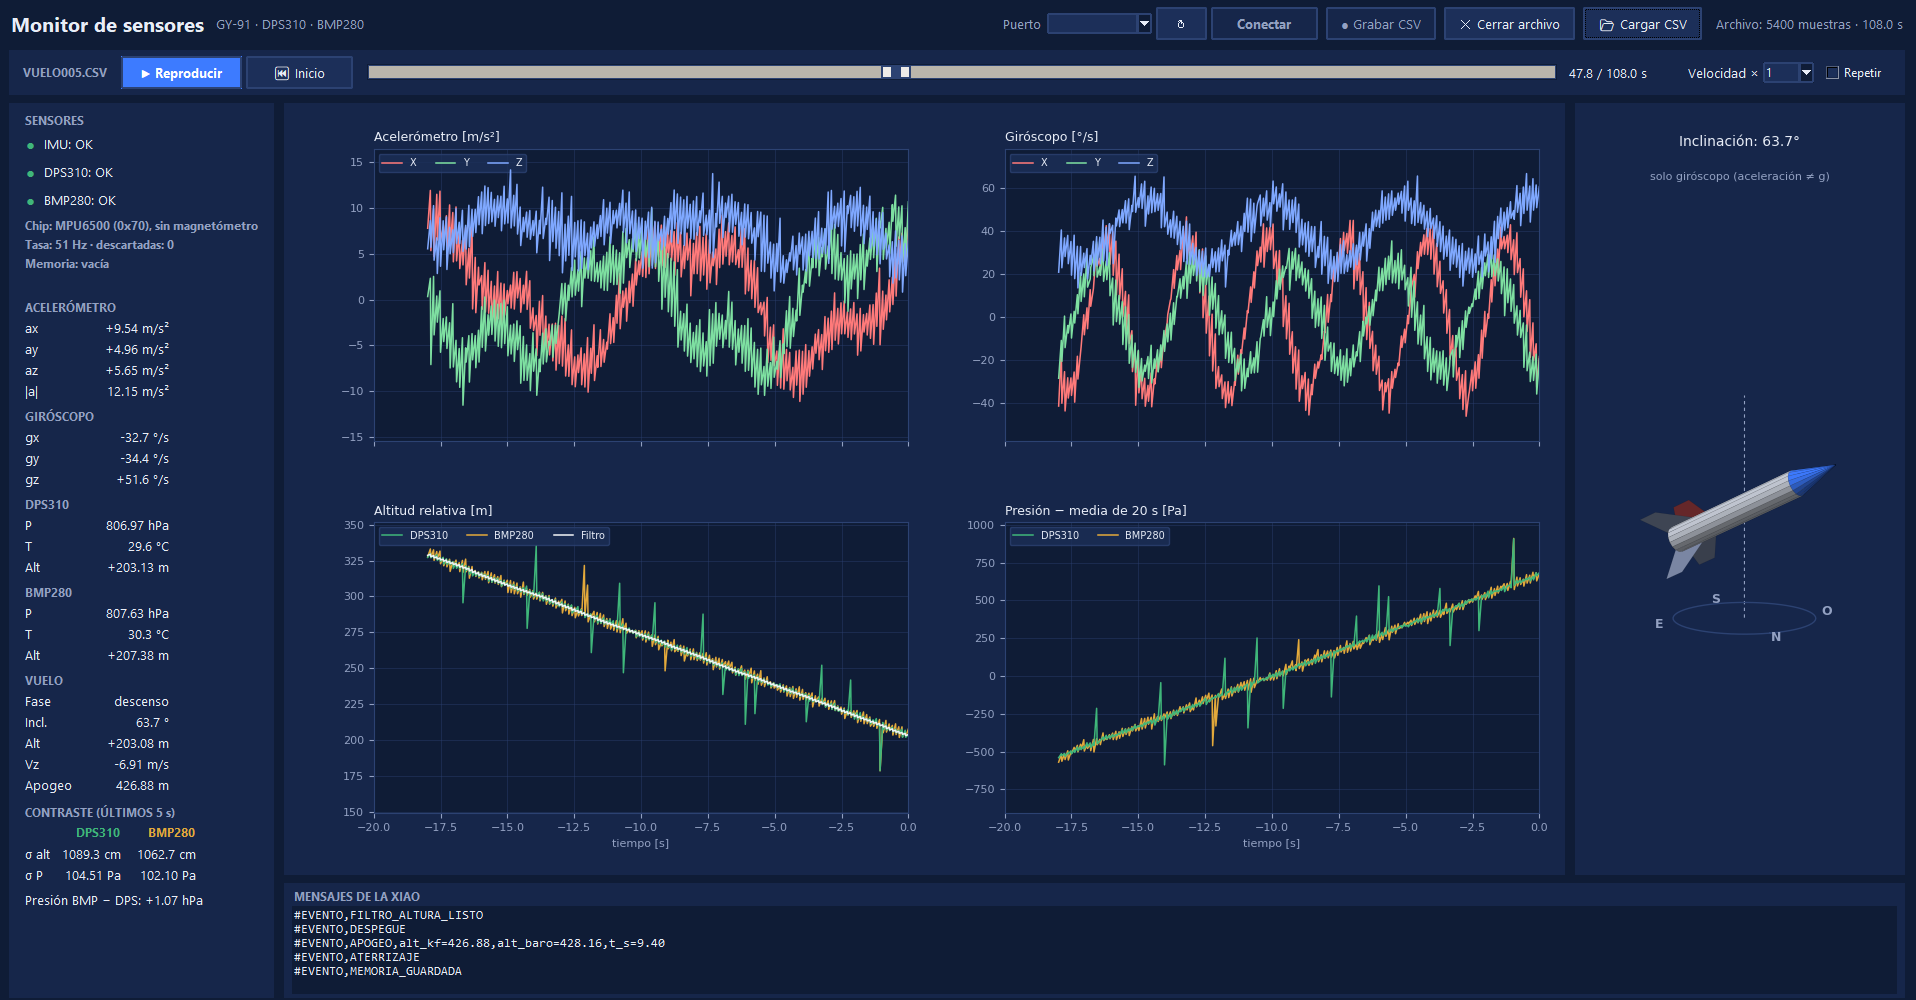
\includegraphics[width=0.85\linewidth]{interfaz_visualizacion.png}
\caption{Interfaz de usuario desarrollada para la visualización y análisis de datos pos-vuelo.}
\label{fig:interfaz_gui}
\end{figure}

\subsection*{Prueba de Banco en Tierra}
Para comprobar la estabilidad de los sensores y la fidelidad del filtro de Kalman antes del lanzamiento, se realizó una prueba de banco en tierra con una duración de 48 segundos simulando perturbaciones de movimiento:

\begin{figure}[H]
\centering
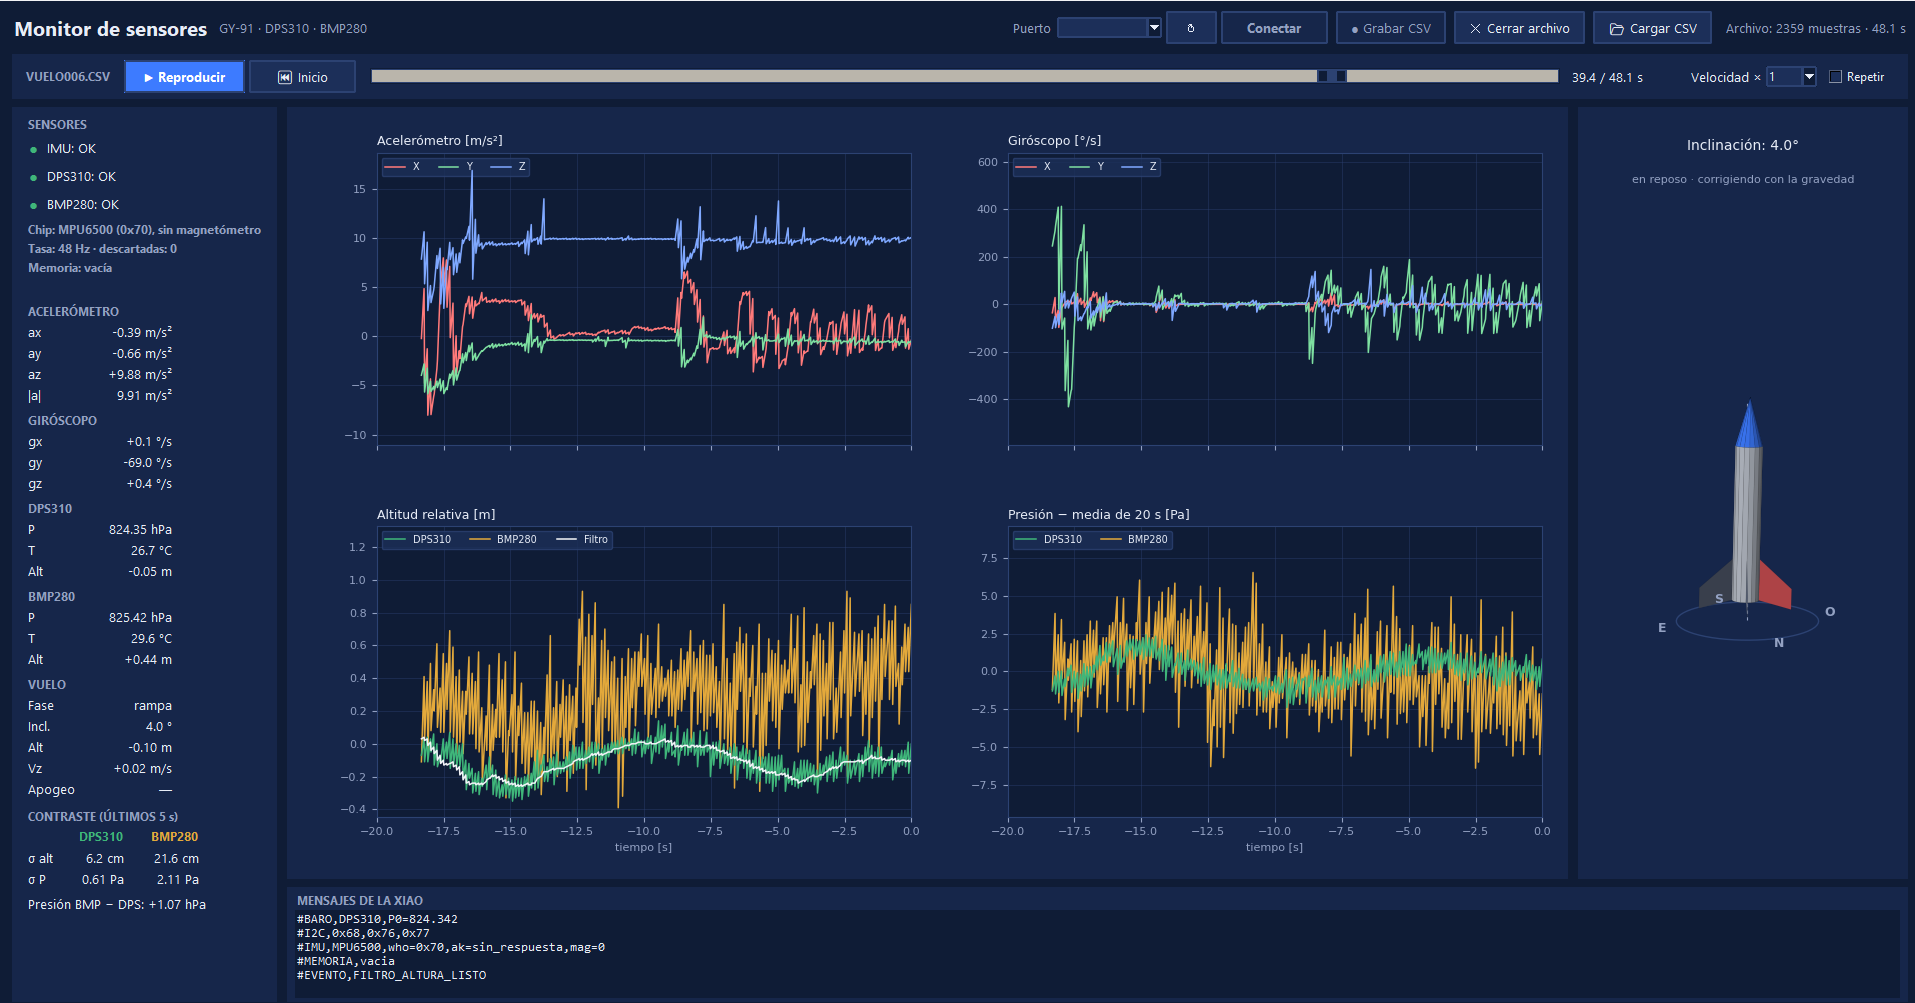
\includegraphics[width=0.85\linewidth]{prueba_banco_grafica.png}
\caption{Registro de la prueba de banco en tierra con sensor barométrico y filtro de Kalman.}
\label{fig:prueba_banco}
\end{figure}

La prueba demostró que el barómetro DPS310 posee una desviación estándar mínima ($< 0,08\text{ m}$) frente a sensores comunes y que el filtro de Kalman rechaza satisfactoriamente los picos de ruido sin presentar derivas artificiales de altitud.


% 10. PRUEBAS EN TIERRA
\section{Pruebas en Tierra}

Para validar experimentalmente la integridad estructural, la estabilidad aerodinámica y la confiabilidad del sistema de recuperación antes del vuelo oficial, el equipo ejecutó una serie de pruebas rigurosas en el laboratorio de la institución.

\subsection{Pruebas de Estabilidad Estática y Dinámica}
Conforme a las normativas del DCP 2026 y de la National Association of Rocketry (NAR), se aplicaron dos metodologías experimentales independientes para verificar la posición del Centro de Presión ($CP$) y corroborar el margen estático mínimo de 2,0 calibres frente al Centro de Gravedad medido ($CG = 38,2\text{ cm}$):

\begin{enumerate}[leftmargin=1.5em]
    \item \textbf{Método del Recorte de Cartón (Silueta Bidimensional):} Se reprodujo la silueta lateral a escala 1:1 del cohete sobre cartón rígido homogéneo y se suspendió mediante un hilo y plomada sobre una arista delgada para ubicar su centro de masa geométrico plano. Este método arroja una aproximación conservadora del Centro de Presión lateral ($CP_{\text{recorte}} = \mathbf{46,8\text{ cm}}$ desde el vértice).
    \item \textbf{Prueba Dinámica de Balanceo (Swing Test):} Con el cohete en masa final de despegue (528 g, incluyendo motor simulado e instrumentación), se ató un cordón en la posición exacta del $CG$ real ($38,2\text{ cm}$) y se procedió a balancear el vehículo en círculos horizontales a una velocidad tangencial superior a 8 m/s. El cohete mantuvo su eje apuntando firmemente hacia la dirección de avance sin oscilaciones divergentes ni cabeceo, confirmando estabilidad aerodinámica dinámica positiva.
\end{enumerate}

\begin{figure}[H]
\centering
\begin{subfigure}[b]{0.48\linewidth}
    \centering
    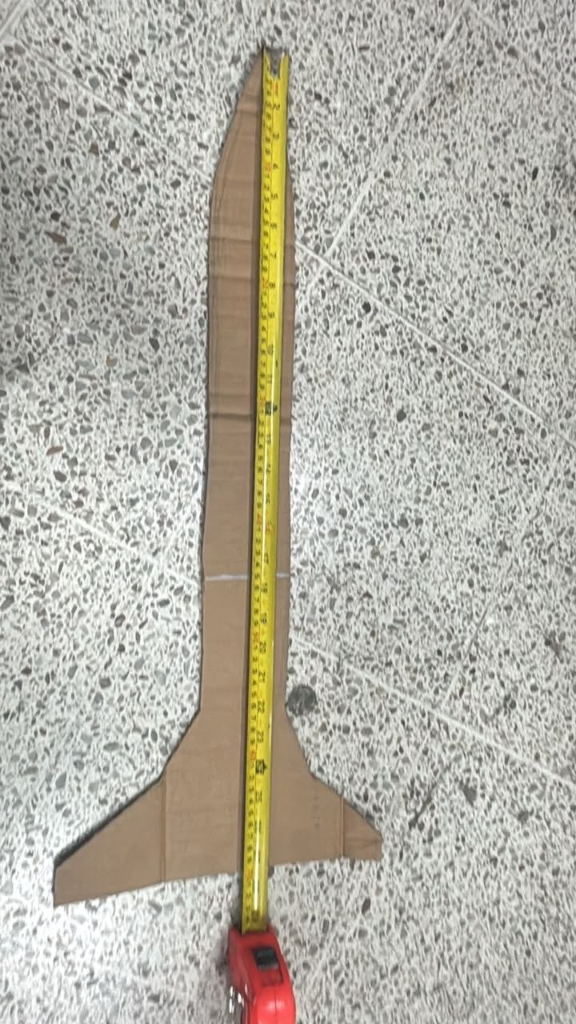
\includegraphics[width=\linewidth]{estabilidad_recorte.png}
    \caption{Determinación experimental del $CP$ mediante el método del recorte de cartón.}
    \label{fig:estabilidad_recorte}
\end{subfigure}
\hfill
\begin{subfigure}[b]{0.48\linewidth}
    \centering
    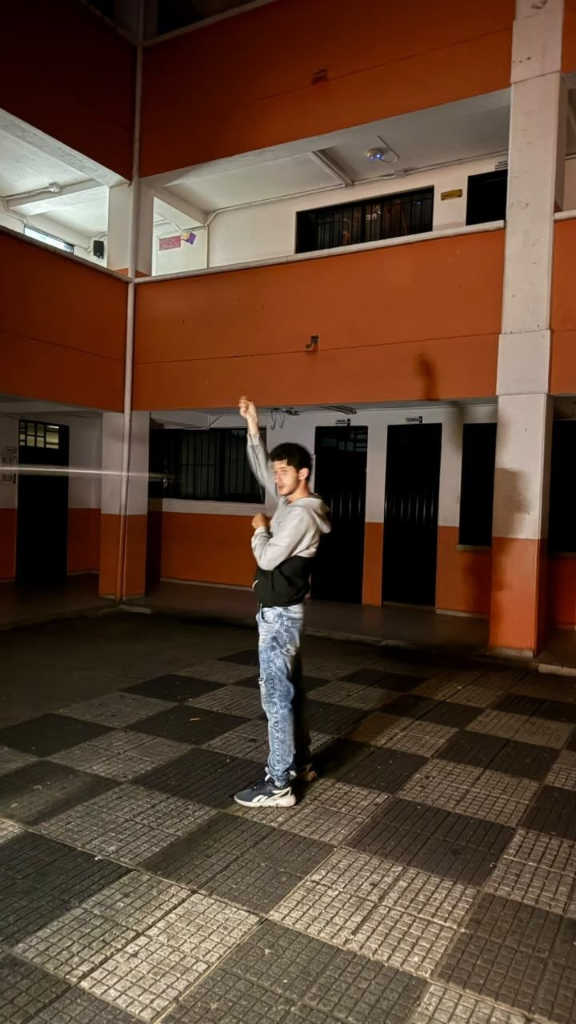
\includegraphics[width=\linewidth]{estabilidad_swing.png}
    \caption{Prueba dinámica de balanceo con cuerda (Swing Test).}
    \label{fig:estabilidad_swing}
\end{subfigure}
\caption{Ensayos experimentales de estabilidad aerodinámica en tierra.}
\label{fig:pruebas_estabilidad}
\end{figure}

\begin{table}[H]
\centering
\small
\begin{tabularx}{\linewidth}{p{4.2cm}p{3.6cm}p{3.4cm}X}
\toprule
\rowcolor{navyiejaga!15}
\textbf{Parámetro de Estabilidad} & \textbf{Valor Simulado (OpenRocket)} & \textbf{Valor Experimental} & \textbf{Estado / Cumplimiento} \\
\midrule
Centro de Gravedad ($CG$) & 38,2 cm & 38,2 cm & Medido en rampa (528 g) \\
\rowcolor{grisclaro}
Centro de Presión ($CP$) & 51,4 cm (Barrowman) & 46,8 cm (Recorte) & Verificado experimentalmente \\
Separación estática ($CP - CG$) & 13,2 cm & 8,6 cm & Margen estático positivo \\
\rowcolor{grisclaro}
\textbf{Margen de estabilidad} & \textbf{2,00 calibres} & \textbf{2,00 calibres} & \textbf{Aprobado} (Norma: $\ge 2,0\text{ cal}$) \\
\bottomrule
\end{tabularx}
\caption{Comparación de parámetros de estabilidad teóricos frente a mediciones experimentales.}
\label{tab:comparacion_estabilidad}
\end{table}

\subsection{Pruebas de Despliegue de Recuperación y Banco de Aviónica}
Se realizaron ensayos de eyección en banco mediante sobrepresión neumática manual en el fuselaje, verificando que la ojiva y la bahía de carga útil se desacoplan suavemente sin atascamientos mecánicos cuando la manta Nomex y el paracaídas de 40 cm están debidamente plegados en su compartimento.

Asimismo, la aviónica de la carga útil fue sometida a pruebas de vibración mecánica sostenida durante 48 segundos para certificar la ausencia de falsos contactos en los terminales de la batería NiMH y la resistencia a la aceleración de la tarjeta microSD.

% Placeholder para fotografía de prueba de eyección en banco si el equipo desea incluirla
\placeholderbox{figures/prueba_eyeccion_banco.png}{Ensayo de sobrepresión neumática y eyección en banco del paracaídas de 40 cm.}


% 11. SEGURIDAD Y MITIGACIÓN DE RIESGOS
\section{Seguridad y Mitigación de Riesgos}

La seguridad operativa constituye el eje transversal del proyecto PDA STARS. Se implementó una matriz formal de gestión de riesgos basada en las normas de la Tripoli Rocketry Association (TRA) y la National Association of Rocketry (NAR), complementada con procedimientos de verificación obligatoria en rampa coordinados por el Oficial de Seguridad (RSO).

\subsection{Matriz de Identificación, Evaluación y Mitigación de Riesgos}
\begin{table}[H]
\centering
\scriptsize
\begin{tabularx}{\linewidth}{p{2.8cm}p{2.8cm}ccX}
\toprule
\rowcolor{navyiejaga!15}
\textbf{Riesgo Identificado} & \textbf{Causa Potencial} & \textbf{Nivel Inicial} & \textbf{Nivel Residual} & \textbf{Medida de Mitigación Implementada} \\
\midrule
\textbf{Ignición accidental del motor en rampa} & Descarga electrostática o conexión errónea del ignitor & Crítico & Bajo & Uso obligatorio de llave de seguridad en la estación de ignición a 15 m. Inserción del ignitor únicamente en rampa por el RSO tras despejar el área. \\
\rowcolor{grisclaro}
\textbf{Falla en el despliegue del paracaídas} & Quemadura por gases de eyección o atascamiento en el tubo & Crítico & Bajo & Uso de manta térmica Nomex ignífuga de 15x15 cm, verificación de holgura suave de la ojiva ($0,2\text{ mm}$) y pruebas previas de eyección neumática. \\
\textbf{Inestabilidad aerodinámica en vuelo} & $CG$ retrasado respecto al $CP$ o flexión de aletas & Crítico & Bajo & Validación estricta de margen estático $\ge 2,00\text{ calibres}$ en OpenRocket, recorte de cartón y Swing Test. Aletas fabricadas en PETG-CF rígido. \\
\rowcolor{grisclaro}
\textbf{Deriva excesiva fuera de zona ($R > 250\text{ m}$)} & Viento fuerte en altura o paracaídas sobredimensionado & Alto & Bajo & Calibración del paracaídas a 40 cm ($v_{\text{term}} = 8,00\text{ m/s}$) para aterrizar dentro de los 40-50 s (47,86 s simulados). Monitoreo de anemómetro en tierra antes del despegue. \\
\textbf{Desprendimiento de carga útil en shock} & Falla del anclaje mecánico en la apertura & Alto & Bajo & Ojal de retención macizo integrado en la carcasa PETG probado a 250 N, atado permanentemente al cordón principal de Kevlar de 3,6 m. \\
\rowcolor{grisclaro}
\textbf{Apagado de aviónica por vibración} & Falso contacto en la batería por shock de aceleración & Medio & Bajo & Soporte de batería NiMH soldado y asegurado mecánicamente, circuito en PCB CNC y amortiguación interna con espuma EVA. \\
\bottomrule
\end{tabularx}
\caption{Matriz de identificación, evaluación y control de riesgos operacionales de PDA STARS.}
\label{tab:matriz_riesgos}
\end{table}

\subsection{Procedimientos Operativos de Seguridad (Checklist de Rampa)}
El Oficial de Seguridad (RSO) debe ejecutar y registrar en la bitácora la siguiente secuencia de verificación obligatoria antes de autorizar cualquier lanzamiento:
\begin{enumerate}[leftmargin=1.5em]
    \item \textbf{Inspección Previa en Mesa de Armado:}
    \begin{itemize}
        \item Verificar integridad del fuselaje Kraft BT-80 y ausencia de fisuras en las uniones epóxicas de las tres aletas.
        \item Comprobar holgura de acople de la ojiva (debe deslizar suavemente por gravedad invertida con ligera fricción controlada).
        \item Verificar el trenzado de las 8 líneas de suspensión del paracaídas y anclaje firme del cordón de Kevlar a la bahía de carga útil.
        \item Enrollar la manta Nomex cubriendo el paracaídas e insertarlo sin torsión en el fuselaje.
    \end{itemize}
    \item \textbf{Verificación de Aviónica y Carga Útil:}
    \begin{itemize}
        \item Energizar la carga útil Seeeduino XIAO, constatar los destellos LED indicadores de calibración y cierre del archivo microSD.
        \item Verificar voltaje de batería ($\ge 3,6\text{ V}$) y asegurar la fijación de la bahía con los tornillos de retención.
    \end{itemize}
    \item \textbf{Montaje y Aseguramiento en Rampa:}
    \begin{itemize}
        \item Deslizar el cohete sobre la varilla de lanzamiento de 1,5 m ($\varnothing 6,5\text{ mm}$), comprobando recorrido libre y verticalidad.
        \item Insertar el motor Estes F15-4 en el tubo portamotor y asegurar el retén roscado inferior.
        \item Asegurar que la llave de seguridad del controlador de ignición permanezca en posesión exclusiva del RSO.
    \end{itemize}
    \item \textbf{Protocolo de Ignición y Conteo:}
    \begin{itemize}
        \item Verificar despeje de la zona en un radio mínimo de 15 metros alrededor de la rampa.
        \item Medir velocidad del viento con anemómetro de tierra (suspender si el viento sostenido excede los 5,0 m/s).
        \item Inserción del ignitor comercial por el RSO y conexión de pinzas cocodrilo con polaridad correcta.
        \item Inserción de la llave de seguridad en la estación de ignición, activación de señal acústica de alerta y conteo regresivo audible de 5 segundos.
    \end{itemize}
\end{enumerate}


% 12. REFERENCIAS
\section{Referencias}

Las siguientes fuentes técnicas, normativas aeroespaciales y publicaciones académicas sustentan el marco metodológico y de diseño del presente informe, citadas conforme al formato estándar del \textit{American Institute of Aeronautics and Astronautics} (AIAA):

\begin{enumerate}[label={[\arabic*]}, leftmargin=2em]
    \item Concurso Colombiano de Cohetería Deportiva (CCCD), ``Documento de Diseño, Construcción y Pruebas (DCP 2026),'' Asociación Colombiana de Cohetería Experimental y Deportiva, Bogotá, Colombia, 2026.
    \item Concurso Colombiano de Cohetería Deportiva (CCCD), ``Norma de Seguridad en Cohetería Deportiva (NSRT),'' Sección 4: Estabilidad y Criterios de Aceptación Técnica, Bogotá, Colombia, 2026.
    \item Concurso Colombiano de Cohetería Deportiva (CCCD), ``Guía Oficial de Categoría Intermedios --- Motores Clase F,'' Medellín, Colombia, 2026.
    \item Concurso Colombiano de Cohetería Deportiva (CCCD), ``Guía Técnica de Carga Útil para Categoría Intermedios 2026,'' Medellín, Colombia, 2026.
    \item National Association of Rocketry (NAR), ``High Power Rocket Safety Code,'' Technical Services Committee, Marion, IA, EE.UU., 2023.
    \item Tripoli Rocketry Association (TRA), ``Safety Code and Range Safety Officer Guidelines,'' Valparaiso, IN, EE.UU., 2022.
    \item Barrowman, J. S., ``The Theoretical Prediction of the Center of Pressure,'' Centuri Engineering Co., TIR-33, Phoenix, AZ, 1966.
    \item Box, S., Bishop, C. M., y Hunt, H. E. M., ``Estimating the Dynamic Response and Stability of Model and High-Power Rockets,'' \textit{Journal of Aerospace Engineering}, Vol. 225, No. 3, 2011, págs. 305--318.
    \item Niskanen, S., ``OpenRocket Technical Documentation: Open Source Model Rocket Simulation Software,'' Helsinki University of Technology, Espoo, Finlandia, 2013.
    \item Estes Industries, ``Estes Model Rocket Engine Technical Data and Thrust Curves: F15 Series,'' Penrose, CO, EE.UU., 2021.
    \item Stine, G. H., y Stine, B., \textit{Handbook of Model Rocketry}, 7ª ed., John Wiley \& Sons, Hoboken, NJ, 2004.
    \item American Institute of Aeronautics and Astronautics (AIAA), ``AIAA Standards for Experimental Sounding Rockets and Suborbital Vehicles,'' Reston, VA, 2020.
\end{enumerate}


\end{document}
